% Options for packages loaded elsewhere
\PassOptionsToPackage{unicode}{hyperref}
\PassOptionsToPackage{hyphens}{url}
%
\documentclass[
]{book}
\usepackage{lmodern}
\usepackage{amsmath}
\usepackage{ifxetex,ifluatex}
\ifnum 0\ifxetex 1\fi\ifluatex 1\fi=0 % if pdftex
  \usepackage[T1]{fontenc}
  \usepackage[utf8]{inputenc}
  \usepackage{textcomp} % provide euro and other symbols
  \usepackage{amssymb}
\else % if luatex or xetex
  \usepackage{unicode-math}
  \defaultfontfeatures{Scale=MatchLowercase}
  \defaultfontfeatures[\rmfamily]{Ligatures=TeX,Scale=1}
\fi
% Use upquote if available, for straight quotes in verbatim environments
\IfFileExists{upquote.sty}{\usepackage{upquote}}{}
\IfFileExists{microtype.sty}{% use microtype if available
  \usepackage[]{microtype}
  \UseMicrotypeSet[protrusion]{basicmath} % disable protrusion for tt fonts
}{}
\makeatletter
\@ifundefined{KOMAClassName}{% if non-KOMA class
  \IfFileExists{parskip.sty}{%
    \usepackage{parskip}
  }{% else
    \setlength{\parindent}{0pt}
    \setlength{\parskip}{6pt plus 2pt minus 1pt}}
}{% if KOMA class
  \KOMAoptions{parskip=half}}
\makeatother
\usepackage{xcolor}
\IfFileExists{xurl.sty}{\usepackage{xurl}}{} % add URL line breaks if available
\IfFileExists{bookmark.sty}{\usepackage{bookmark}}{\usepackage{hyperref}}
\hypersetup{
  pdftitle={Основы геоинформатики},
  pdfauthor={Балтыжакова Татьяна},
  hidelinks,
  pdfcreator={LaTeX via pandoc}}
\urlstyle{same} % disable monospaced font for URLs
\usepackage{longtable,booktabs}
\usepackage{calc} % for calculating minipage widths
% Correct order of tables after \paragraph or \subparagraph
\usepackage{etoolbox}
\makeatletter
\patchcmd\longtable{\par}{\if@noskipsec\mbox{}\fi\par}{}{}
\makeatother
% Allow footnotes in longtable head/foot
\IfFileExists{footnotehyper.sty}{\usepackage{footnotehyper}}{\usepackage{footnote}}
\makesavenoteenv{longtable}
\usepackage{graphicx}
\makeatletter
\def\maxwidth{\ifdim\Gin@nat@width>\linewidth\linewidth\else\Gin@nat@width\fi}
\def\maxheight{\ifdim\Gin@nat@height>\textheight\textheight\else\Gin@nat@height\fi}
\makeatother
% Scale images if necessary, so that they will not overflow the page
% margins by default, and it is still possible to overwrite the defaults
% using explicit options in \includegraphics[width, height, ...]{}
\setkeys{Gin}{width=\maxwidth,height=\maxheight,keepaspectratio}
% Set default figure placement to htbp
\makeatletter
\def\fps@figure{htbp}
\makeatother
\setlength{\emergencystretch}{3em} % prevent overfull lines
\providecommand{\tightlist}{%
  \setlength{\itemsep}{0pt}\setlength{\parskip}{0pt}}
\setcounter{secnumdepth}{5}
\usepackage{booktabs}
\ifluatex
  \usepackage{selnolig}  % disable illegal ligatures
\fi
\usepackage[]{natbib}
\bibliographystyle{plainnat}

\title{Основы геоинформатики}
\author{Балтыжакова Татьяна}
\date{2021-05-06}

\begin{document}
\maketitle

{
\setcounter{tocdepth}{1}
\tableofcontents
}
\hypertarget{intro}{%
\chapter{Общие сведения}\label{intro}}

Этот практикум сделан на основе прошедшего курса по развитию дополнительных компетенций студентов ``Основы геоинформатики''. Курс построен с использованием открытого ПО QGIS, скачать который можно с \href{https://qgis.org/ru/site/}{официального сайта проекта}

Возможно будет дополняться (но это не точно).

\hypertarget{unfolded}{%
\chapter{Создание карты без специализированного программного обеспечения}\label{unfolded}}

Первое занятие посвящено общим принципам построения карт и созданию карт с помощью сервиса \url{unfolded.ai}.

Этот сервис позволяет делать карты прямо в браузере, для того, чтобы им воспользоваться нужно зарегистрироваться на сайте \url{https://studio.unfolded.ai/home}

Подробно про работу с сервисом я рассказывала на мастер-классе в рамках Дня открытых данных. Запись можно посмотреть ниже.

Для работы можно воспользоваться данными из \href{https://github.com/baltti/opendataday-21}{репозитори}я или \href{https://drive.google.com/file/d/171Ts_FX2DFOojv0ru7ApN0wXWhMFVtcF/view?usp=sharing}{данными}, которые будут применяться для дальнейшей работы в рамках курса. Оба набора аналогичны: они содержат названия сетевых супермаркетов и их координаты (широту и долготу), первый набор для Москвы, второй - для Санкт-Петербурга.

Данные © OpenStreetMap contributors

\hypertarget{basics}{%
\chapter{Создание карты и редактирование стиля}\label{basics}}

\hypertarget{ux434ux43eux431ux430ux432ux43bux435ux43dux438ux435-ux43eux431ux44aux435ux43aux442ux43eux432-ux43dux430-ux43aux430ux440ux442ux443}{%
\section{Добавление объектов на карту}\label{ux434ux43eux431ux430ux432ux43bux435ux43dux438ux435-ux43eux431ux44aux435ux43aux442ux43eux432-ux43dux430-ux43aux430ux440ux442ux443}}

После запуска программы нужно создать новый проект, в котором будут храниться все файлы с добавленными слоями, стилями и макетами.

Новый проект будет выглядеть так.

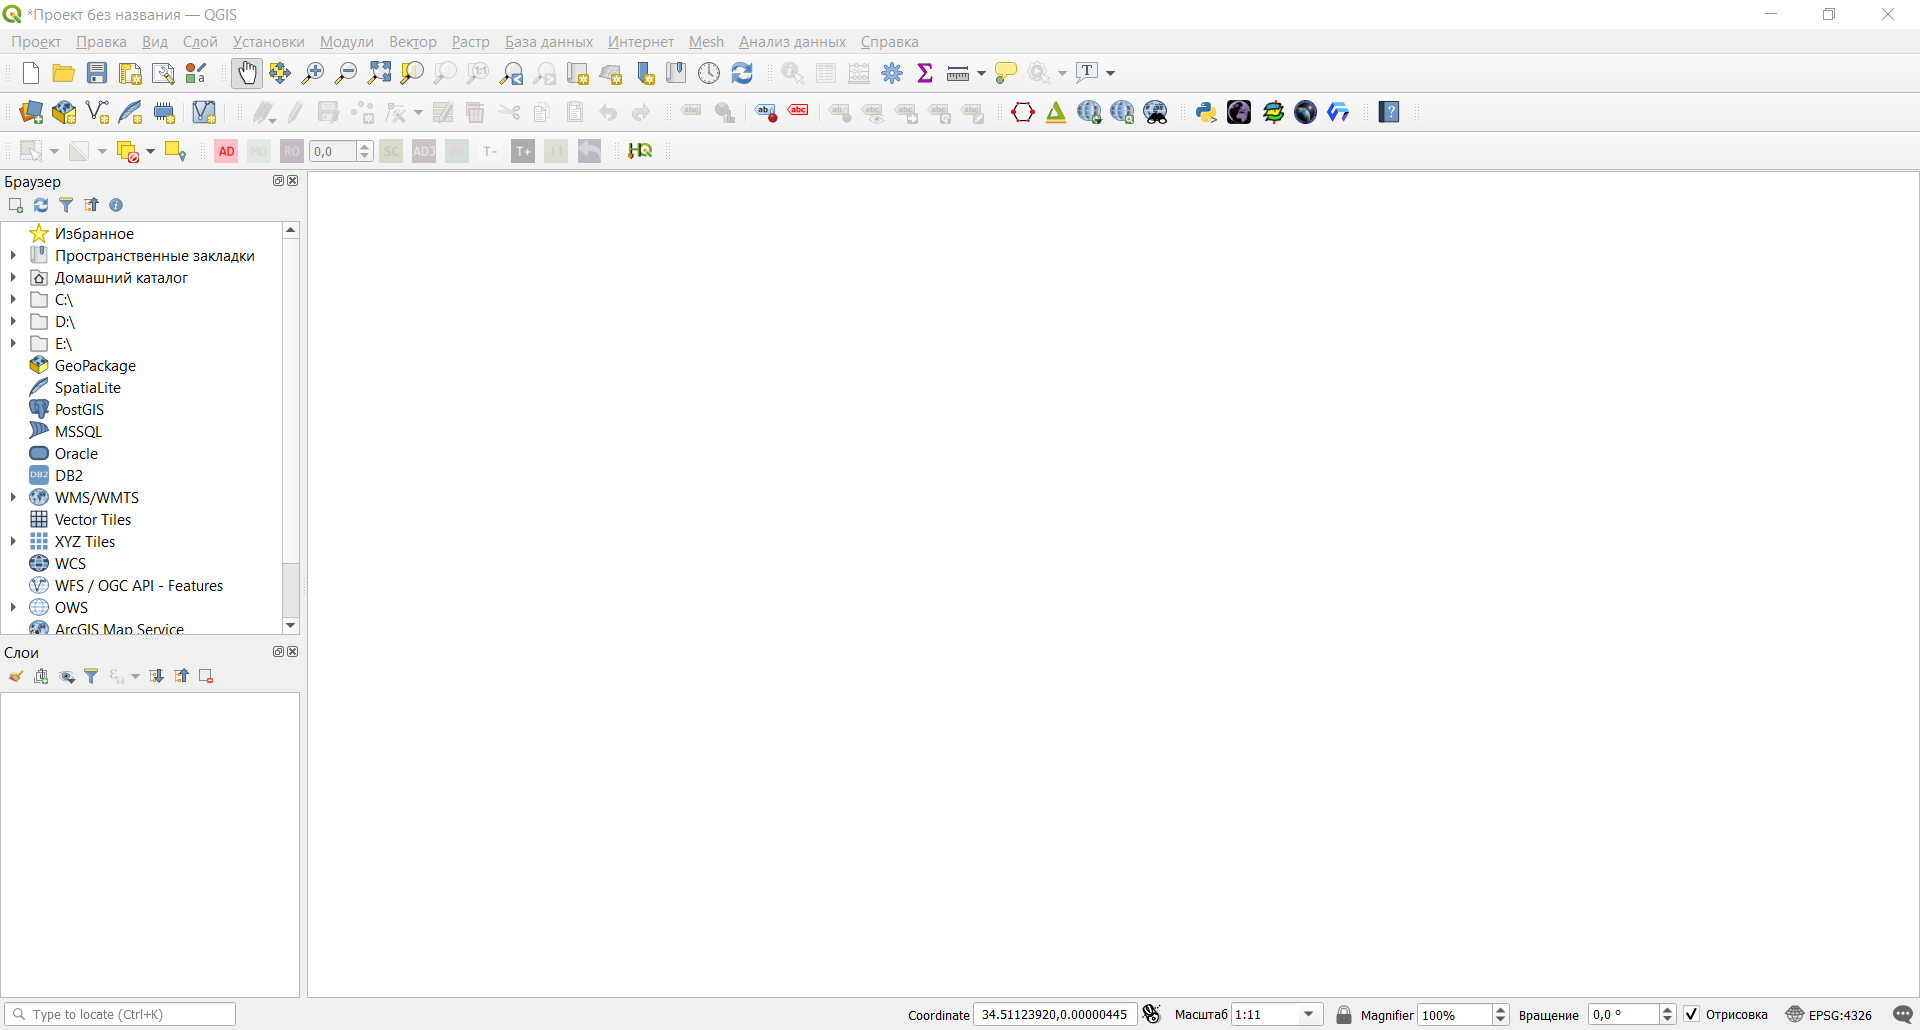
\includegraphics{figures/1.PNG}

Сверху находится строка меню и основная панель инструментов, слева 2 панели: Браузер (здесь отображаются все доступные источники данных) и Слои (здесь будут отображаться все добавленные в проект слои с данными.

Чтобы добавить новый слой из документа в формате csv, нужно в строке меню выбрать \textbf{Слой ⤑Добавить слой⤑Добавить слой из текста с разделителями}.

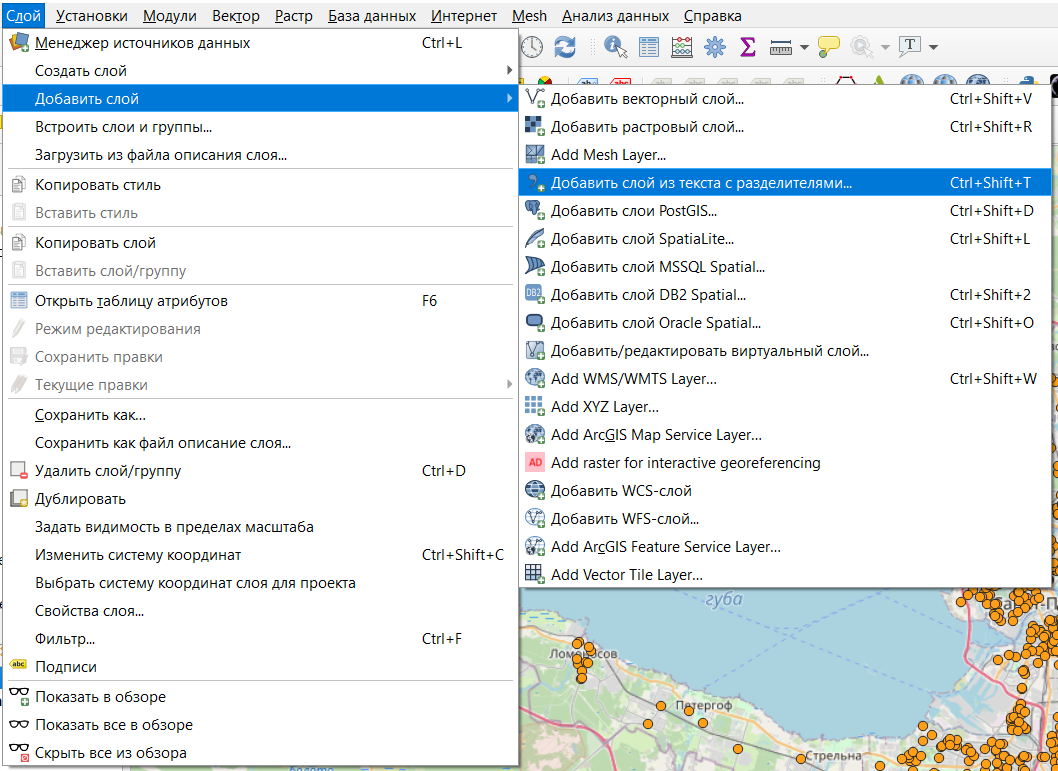
\includegraphics{figures/2.png}

Далее к открывшемся диалоговом окне нужно выбрать файл и установить необходимые настройки

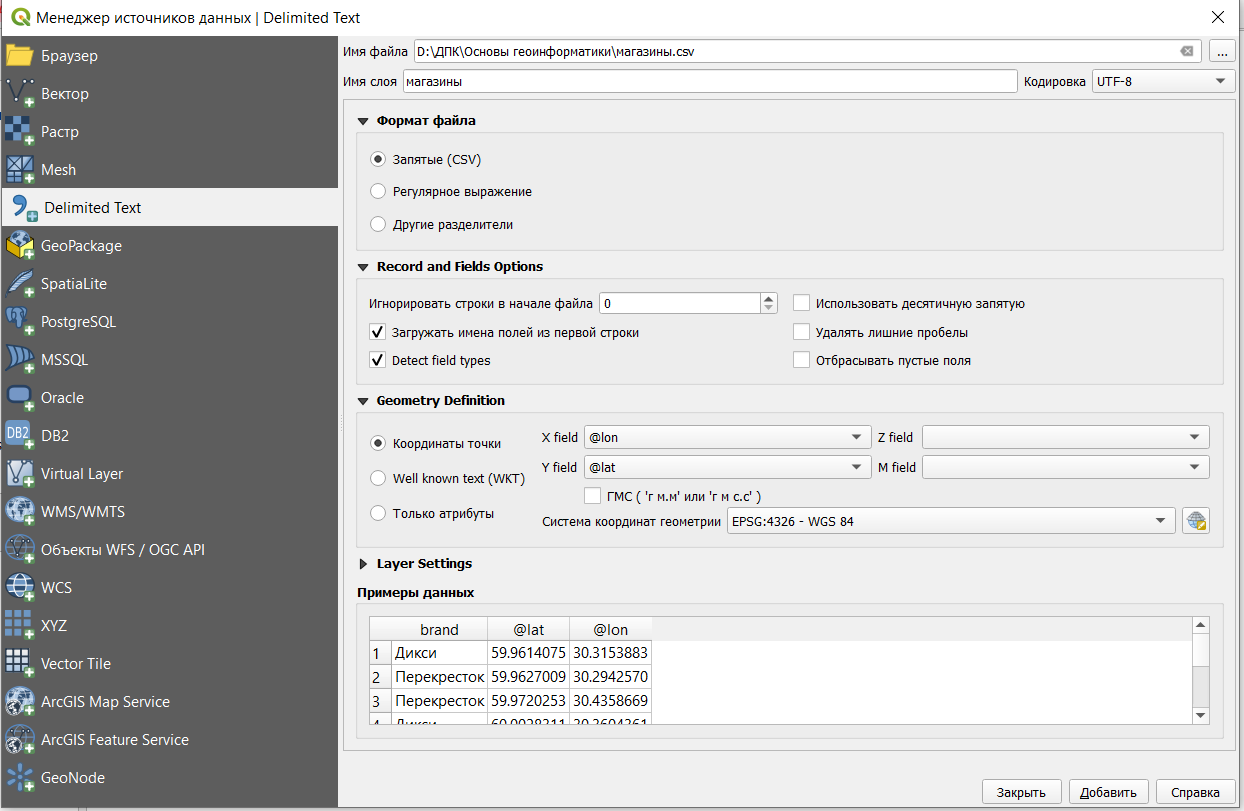
\includegraphics{figures/3.PNG}

Так как координаты объектов в нашем случае заданы широтой и долготой, то необходимо выбрать систему координат \texttt{EPSG:4326\ -\ WGS\ 84} (про системы координат чуть подробнее будет позже) с координатой X - долготой и координатой Y - широтой.

В результате на карте должны появиться точки, нанесенные по координатам.

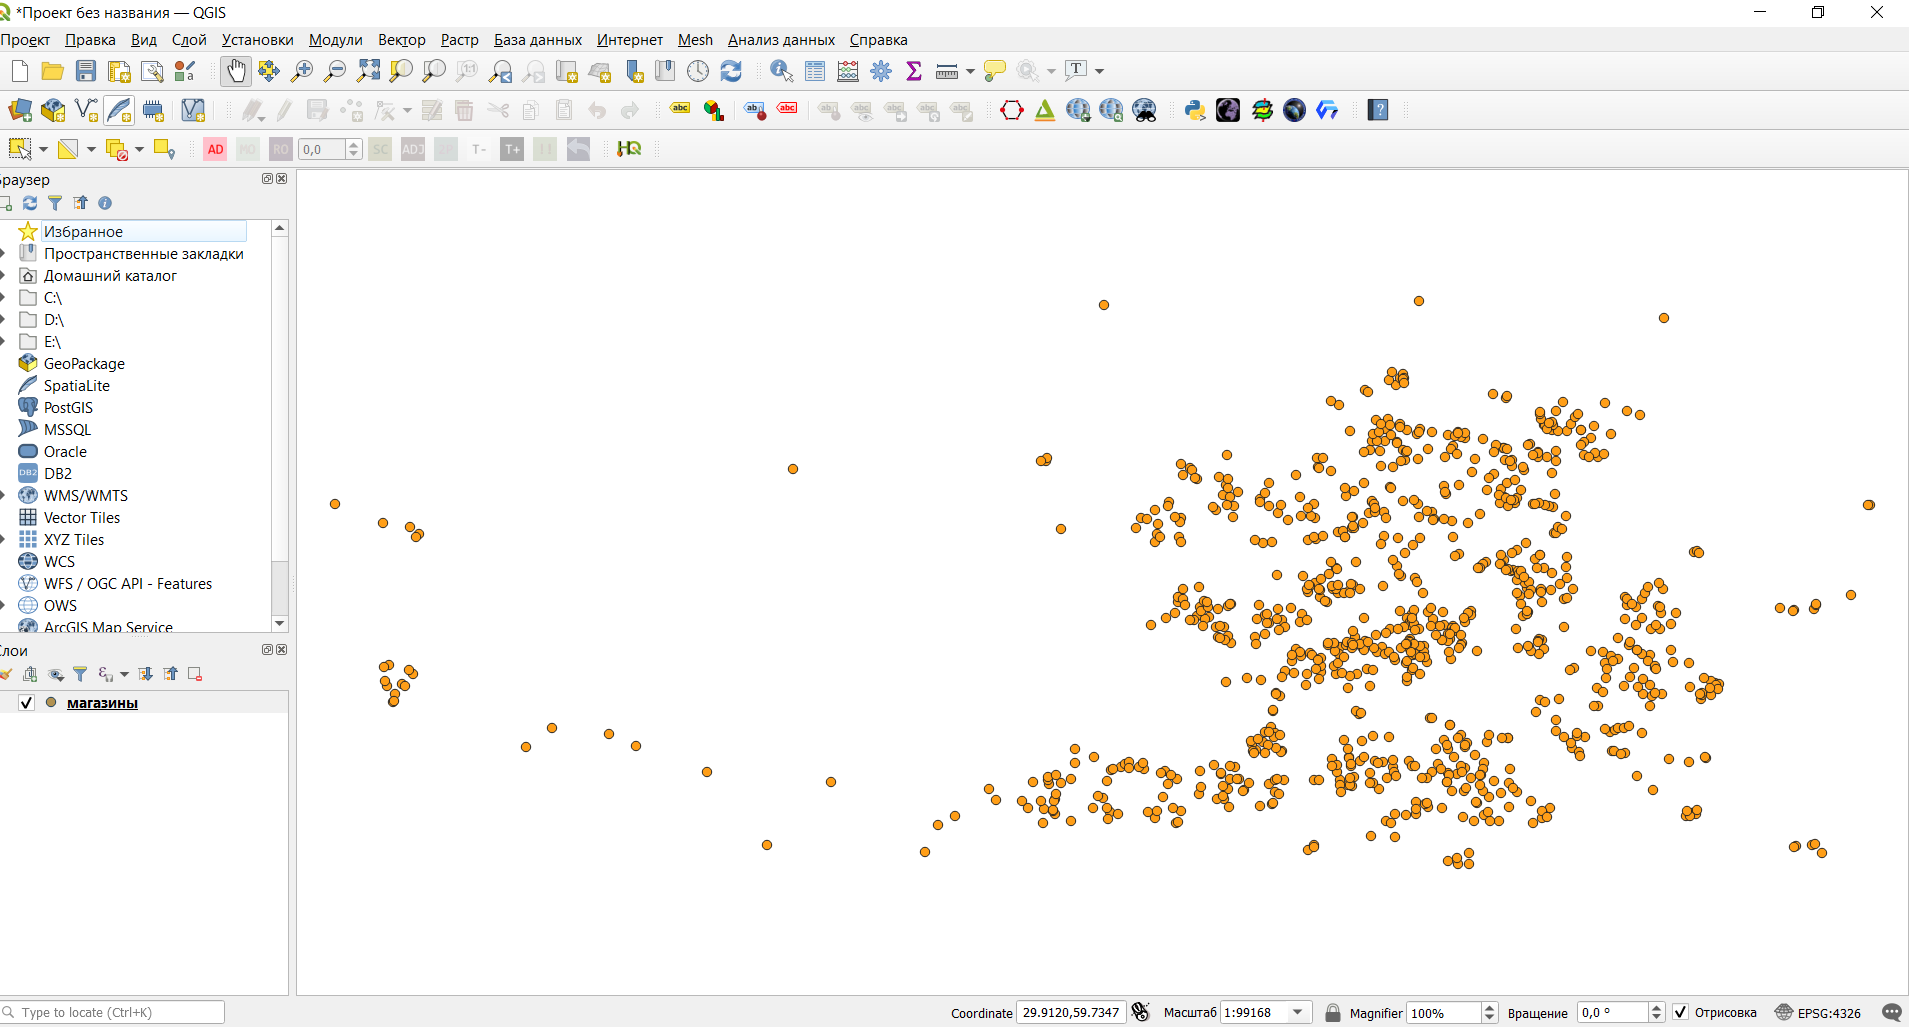
\includegraphics{figures/4.PNG}

Добавим на карту подложку с OpenStreetMap. Она уже содержится в программе по умолчанию, ее можно найти в панели Браузер под названием XYZ Tiles. Чтобы добавить подложку достаточно просто дважды кликнуть по ней.

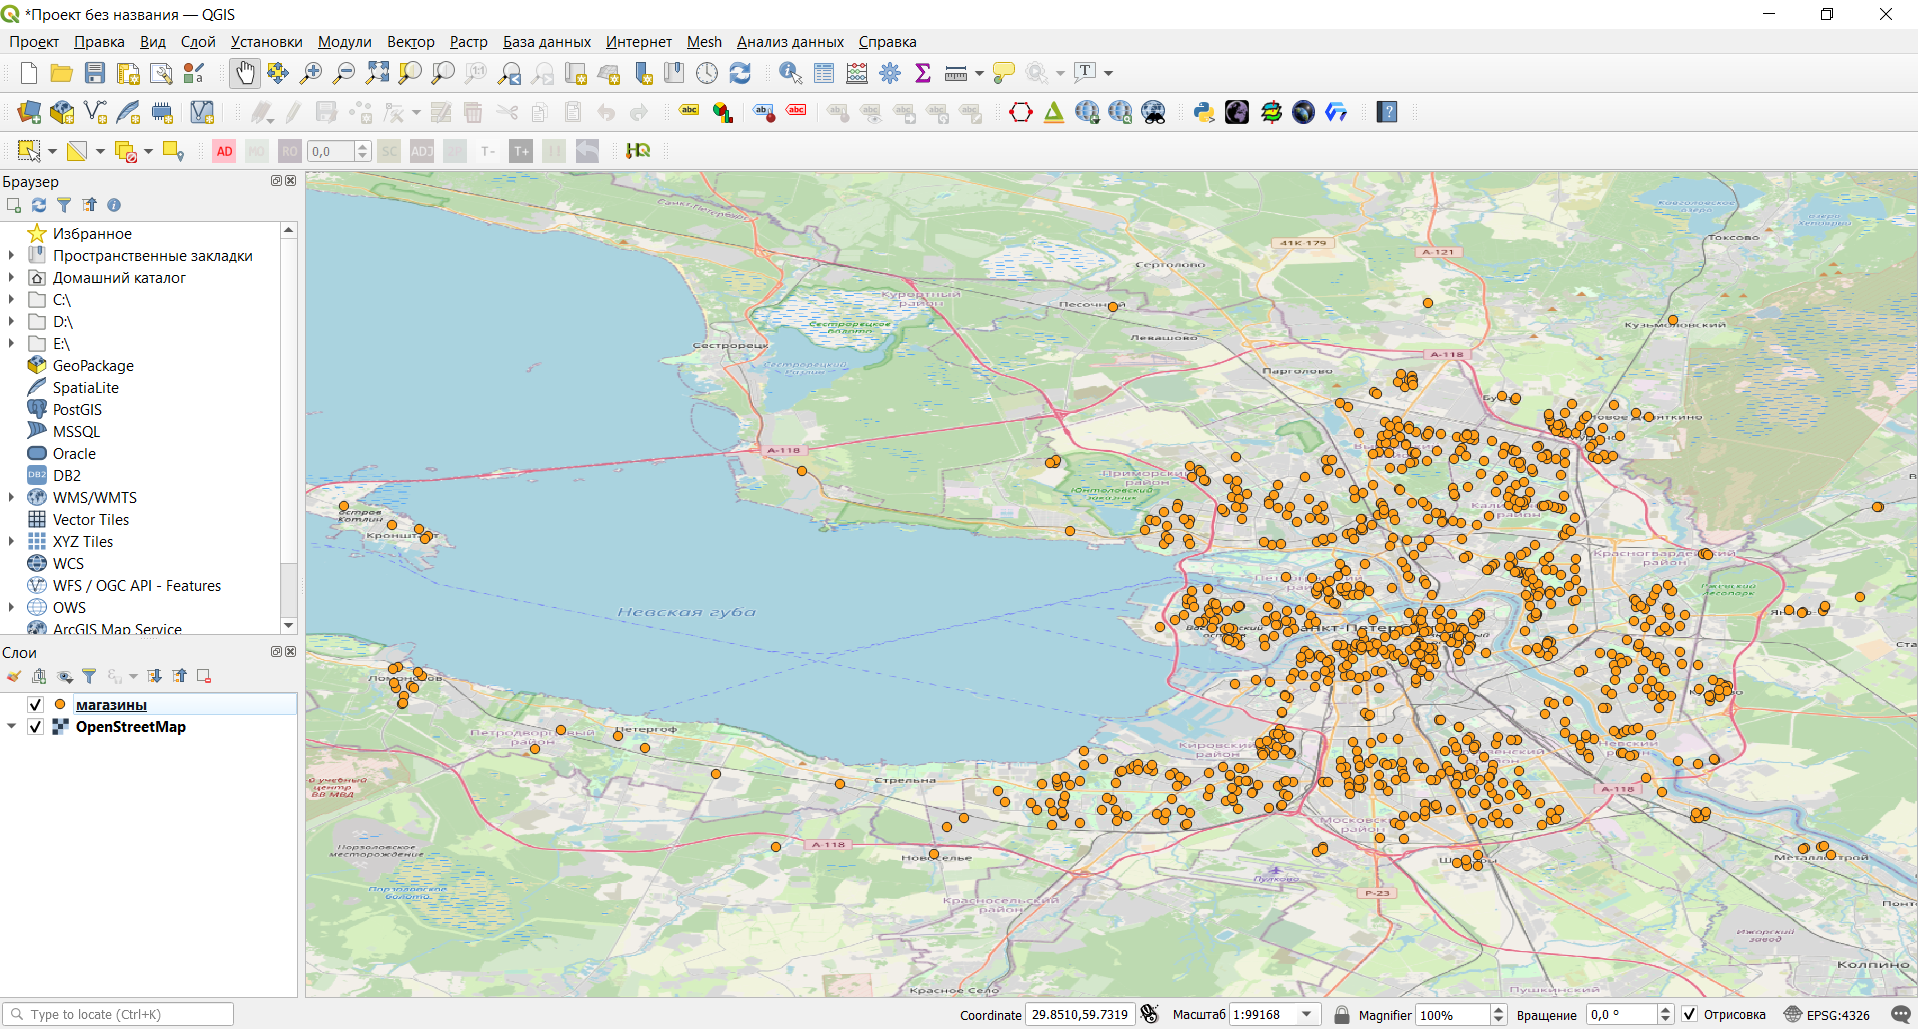
\includegraphics{figures/5.PNG}

Кроме подложки по умолчанию, можно подключить дополнительные тайлы. Для этого нужно щеклнуть правой кнопкой мыши на XYZ Tiles и выбрать пункт \emph{Подключить}. Далее в диалоговом окне обязательно нужно указать имя подключения и ссылку. Можно воспользоваться подложками Google по следуюшим ссылкам:

\begin{itemize}
\item
  карта улиц и дорог \protect\hyperlink{sentux2f_blank}{\underline{http://mt0.google.com/vt/lyrs=m\&hl=en\&x=\{x\}\&y=\{y\}\&z=\{z\}}}
\item
  рельеф \protect\hyperlink{sentux2f_blank}{http://mt0.google.com/vt/lyrs=p\&hl=en\&x=\{x\}\&y=\{y\}\&z=\{z\}}
\item
  модифицированная карта улиц и дорог \protect\hyperlink{sentux2f_blank}{http://mt0.google.com/vt/lyrs=r\&hl=en\&x=\{x\}\&y=\{y\}\&z=\{z\}}
\item
  только спутниковое изображение\protect\hyperlink{sentux2f_blank}{http://mt0.google.com/vt/lyrs=s\&hl=en\&x=\{x\}\&y=\{y\}\&z=\{z\}}
\item
  только рельеф \protect\hyperlink{sentux2f_blank}{http://mt0.google.com/vt/lyrs=t\&hl=en\&x=\{x\}\&y=\{y\}\&z=\{z\}}
\item
  гибридное изображение \protect\hyperlink{sentux2f_blank}{http://mt0.google.com/vt/lyrs=y\&hl=en\&x=\{x\}\&y=\{y\}\&z=\{z\}}
\end{itemize}

Также подложку можно добавить с помощью модуля \emph{QuickMapServices}. Этот модуль нужно предварительно установить с помощью команды из строки меню \textbf{«Модули»→Управление модулями}, далее в открывшемся диалоговом окне в строке поиска набрать название модуля и после нахождения модуля, нажать Установить (Install).

После~установки модуля на панели инструментов появятся две кнопки, с помощью которых можно добавлять в проект подложки из различных сервисов.

Если ранее добавленные точки пропали с карты, нужно просто перетащить их в перечне слоев над подложкой.

Как можно видеть изображение находится как бы под углом. Это объясняется системой координат, установленной по умолчанию. Сделаем перепроецирование карты. Для этого нужно в правом нижнем углу нажать на обозначение системы координат \texttt{EPSG:4326\ -\ WGS\ 84} и далее в открывшемся окне выбрать систему координат \texttt{EPSG:3857\ -\ WGS\ 84\ /\ Pseudo\ Mercator.}

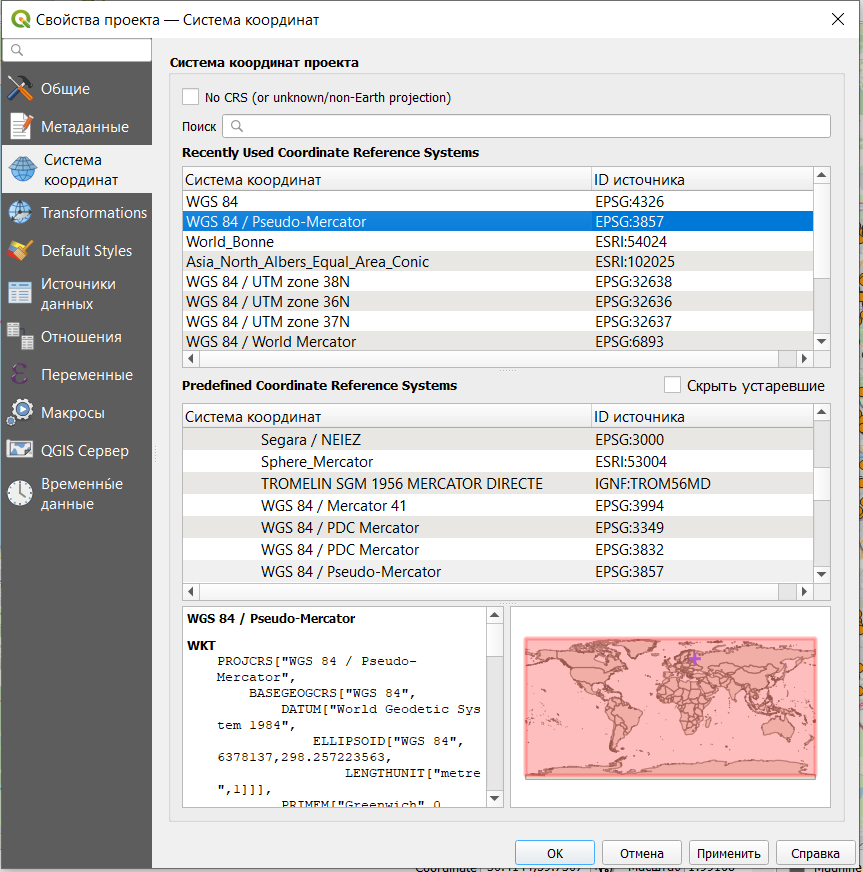
\includegraphics{figures/6.PNG}

Полученный результат будет выглядеть для нас более ``привычным''. Это объясняется тем, что мы выбрали наиболее широко применяемую систему координат в мире: ту, которая используется во всех веб-картах (Google Maps, Yandex и прочие).

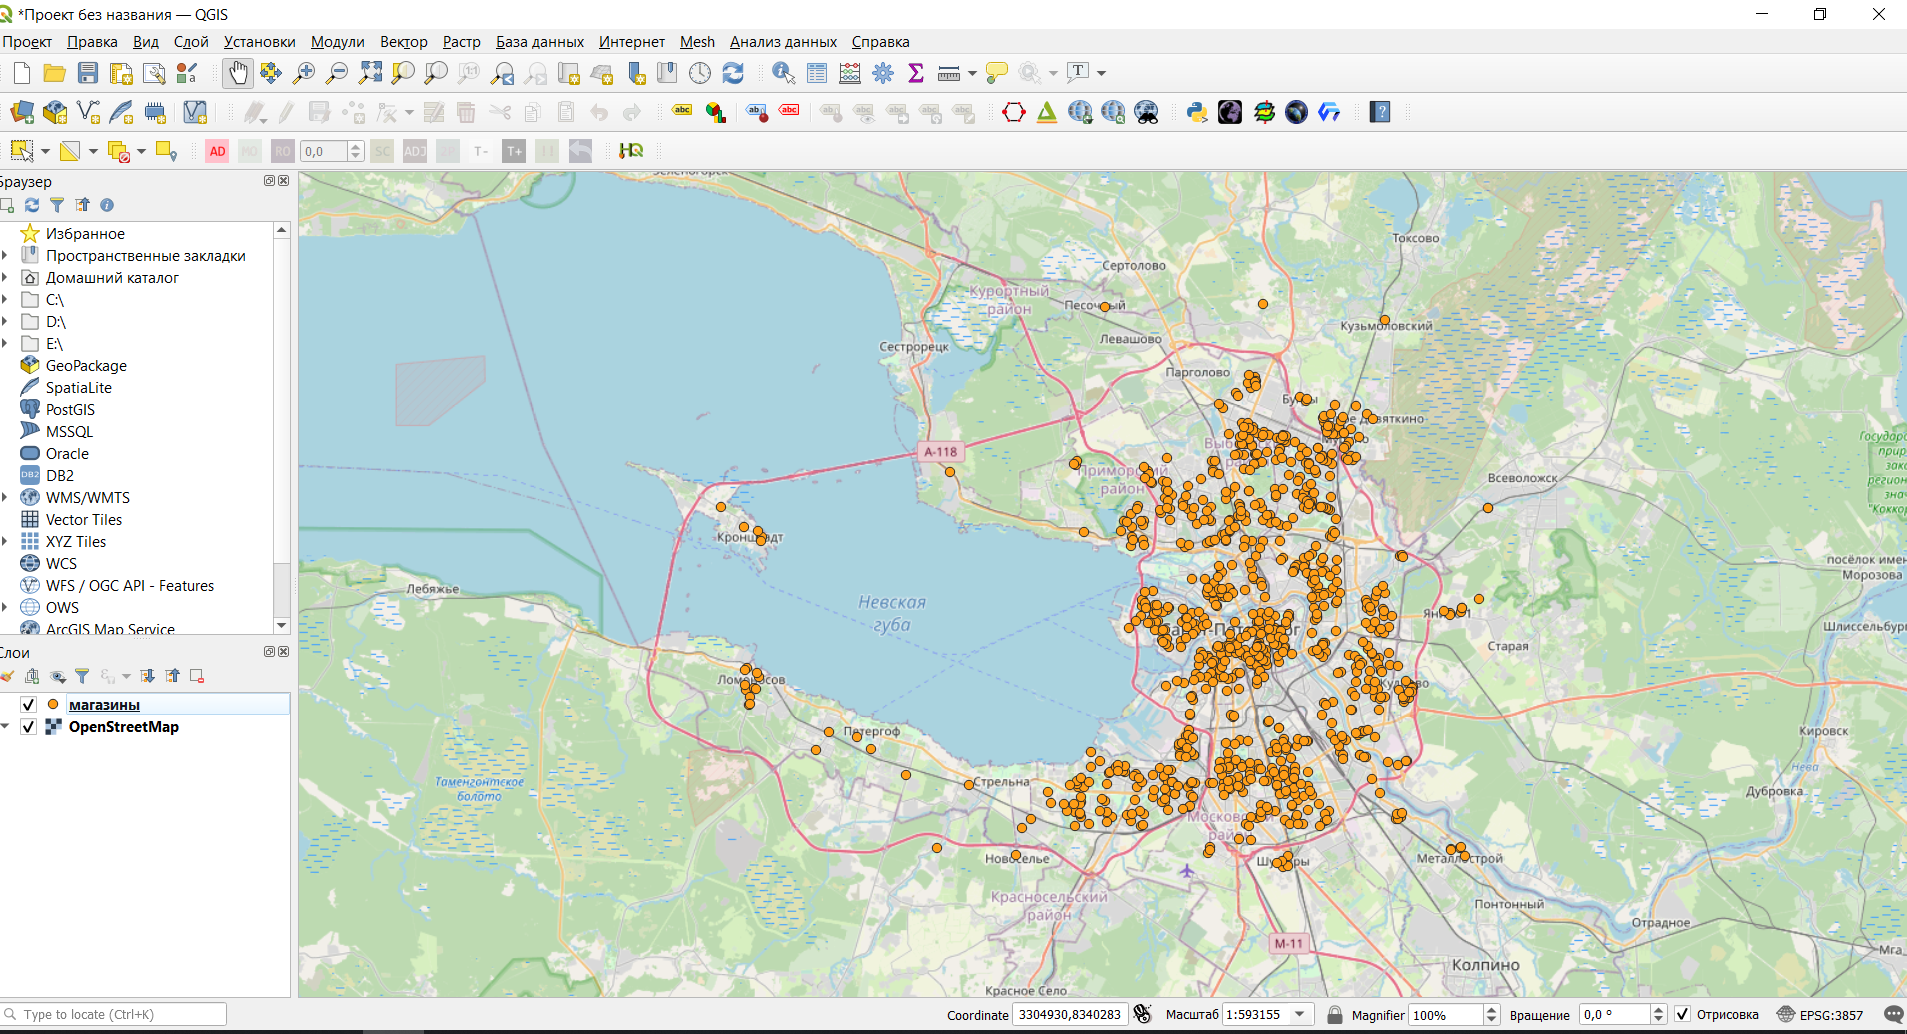
\includegraphics{figures/7.PNG}

\begin{quote}
Важно помнить, что это ``перепроецирование на лету'', которое меняет только отображение данных на карте, проекции слоев остаются в этом случае неизменными. Чтобы изменить проекцию конкретного слоя следует пользоваться инструментом \emph{Перепроецировать слой} из панели инструментов анализа
\end{quote}

\hypertarget{ux441ux438ux441ux442ux435ux43cux44b-ux43aux43eux43eux440ux434ux438ux43dux430ux442}{%
\section{Системы координат}\label{ux441ux438ux441ux442ux435ux43cux44b-ux43aux43eux43eux440ux434ux438ux43dux430ux442}}

При подготовке любых карт одна из самых сложных и важных задач - это подбор правильной проекции. Проекция - это способ отображения поверхности Земли на плоскости.

От выбора проекции зависит степень искажения размеров, длин и углов. Есть мнение, что проекции создают нашу картину мира, о чем есть великий эпизод из сериала West Wing.

Также про проекции есть выпуск веб-комикса \href{https://xkcd.com/977/}{xkcd}.

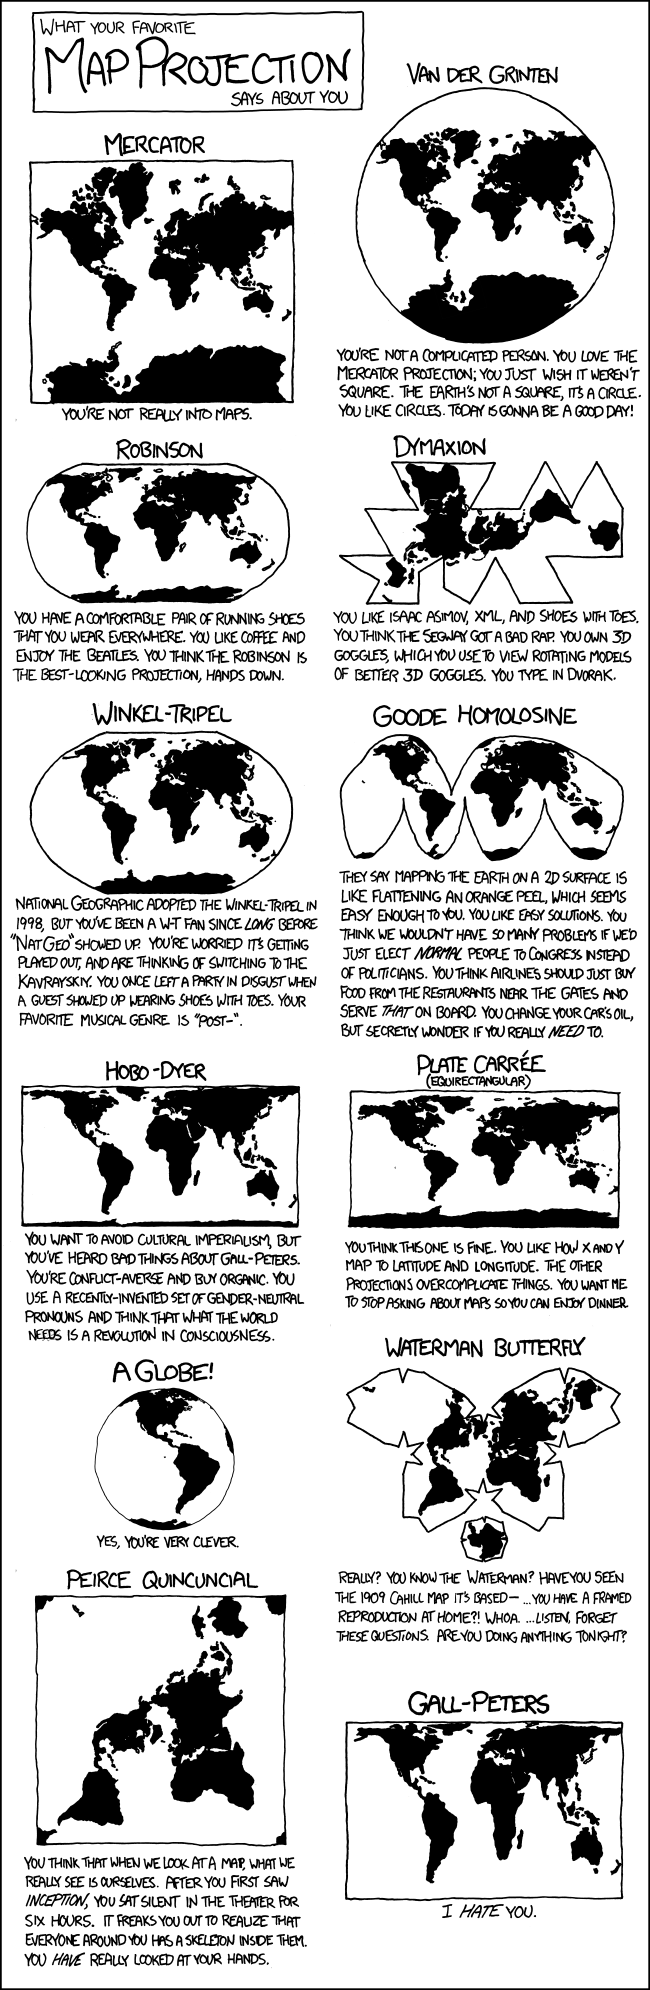
\includegraphics{figures/map_projections.png}

Как уже было сказано чуть выше самой распространенной проекцией, с которой большинство из нас сталкивается практически ежедневно, является \texttt{EPSG:3857\ -\ WGS\ 84\ /\ Pseudo\ Mercator.} В этой проекции очень велики искажения размеров, особенно в приполярных областях, так как она является цилиндрической. То есть при ее создании земной шар помещается внутрь цилиндра, который соприкасается с ним на экваторе, после чего все проецируется на поверхность цилиндра и он разворачивается на плоскость.

Посмотреть, насколько искажаются размеры в привычной нам проекции можно на сайте \href{https://thetruesize.com/}{The True Size \ldots{}}

Но в ГИС все не ограничивается только способом проецирования на плоскость, также важно как и задаются оси координат, где находится начало системы координат, какие единицы измерения используются, каков охват системы координат. Поэтому в ГИС говорят не просто о проекции, а о системе координат - \textbf{coordinate reference system или crs}.

Сейчас используется единая классификация систем координат в ГИС - реестр EPSG, с которым можно ознакомиться на сайте \url{epsg.io}.

Все имеющиеся в реестре системы координат уже заданы в QGIS, а также есть возможность создания пользовательских систем координат. При создании пользовательской системы координат можно составить ее описание в формате \textbf{WKT} (well-known text) или в формате \textbf{proj.}

Для подбора подходящей системы координат можно воспользоваться сервисом \href{http://projectionwizard.org/}{Projection wizard}.

\begin{quote}
Следует помнить, что существует два основных типа систем координат: географические и прямоугольные (спроецированные). В первых в качестве единиц измерения используются градусы, а во вторых - метрические единицы. Это имеет значение при ряде операций пространственного анализа.
\end{quote}

\hypertarget{ux43dux430ux441ux442ux440ux43eux439ux43aux430-ux441ux442ux438ux43bux44f-ux441ux43bux43eux44f}{%
\section{Настройка стиля слоя}\label{ux43dux430ux441ux442ux440ux43eux439ux43aux430-ux441ux442ux438ux43bux44f-ux441ux43bux43eux44f}}

Для того, чтобы настроить стиль слоя, нужно открыть его свойства. Это делается либо двойным щелчком по названию слоя, либо через контекстное меню, вызываемое щелчком правой кнопки мыши по названию слоя.

По умолчанию стиль слоя с точечными объектами задается как \emph{Обычный знак}.

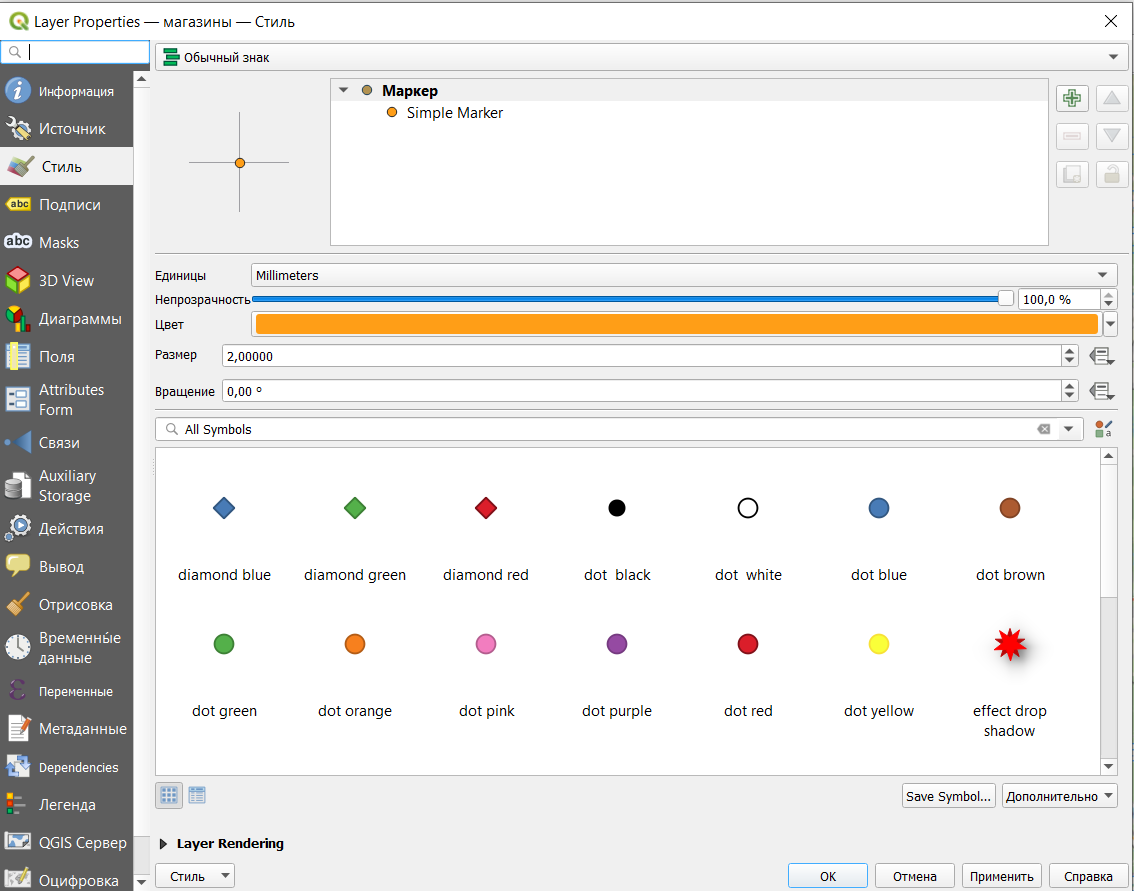
\includegraphics{figures/8.PNG}

Другие доступные варианты

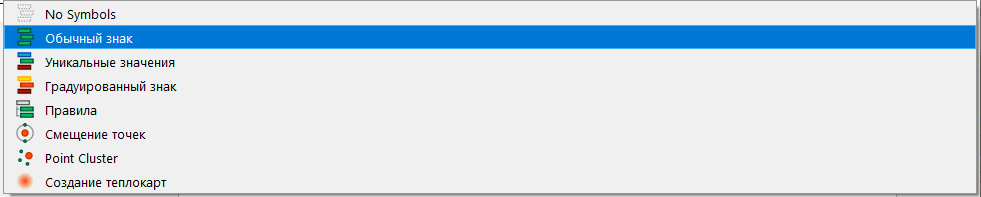
\includegraphics{figures/9.png}

\begin{itemize}
\item
  уникальные значения - как правило, используется для категориальной или дискретной переменной с небольшим количеством значений;
\item
  градуированный знак - для задания символа в зависимости от числовой переменной;
\item
  правила - позволяет задавать символику на основе выражения;
\item
  смещение точек - позволяет показать все точки слоя, даже если они находятся в одном месте, возможны варианты смещения по кругу, концетрическим кругам и сетке;
\item
  point cluster - собирает близко расположенные точечные объекты в один;
\item
  создание теплокарт - создает динамическую карту плотности распределения объектов.
\end{itemize}

Для линейных и площадных объектов настройки стиля будут аналогичны, но не полностью.

Так как в нашем датасете содержится информация о сетевых магазинах самый простой способ стилизовать слой - это уникальные значение по названиям сетей.

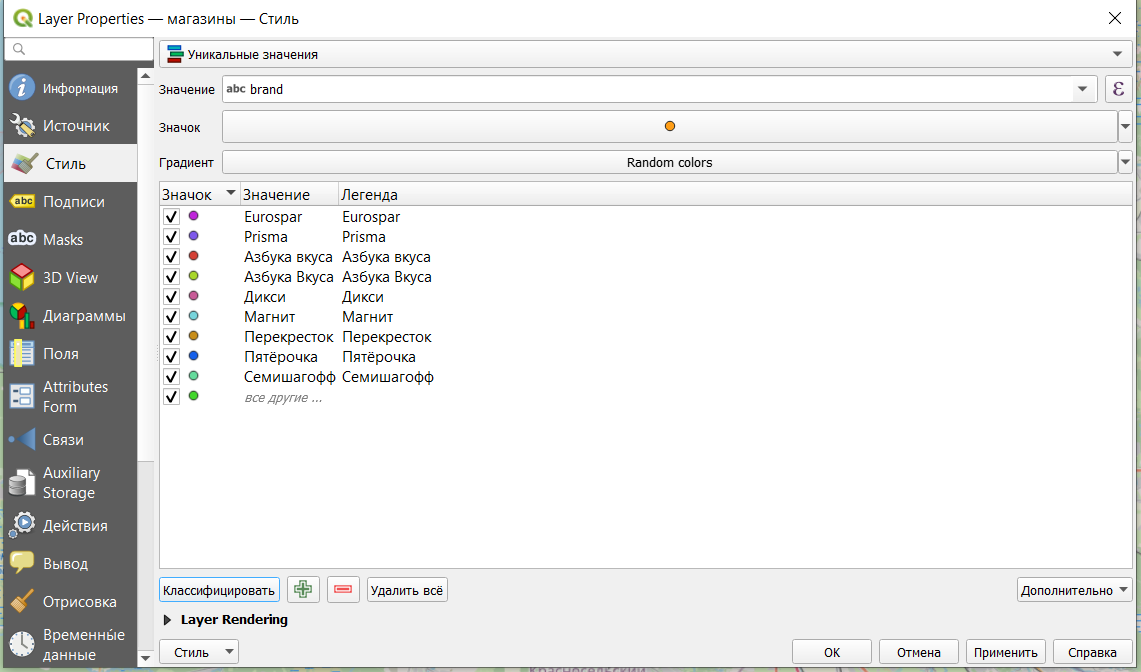
\includegraphics{figures/10.PNG}

После изменения стиля точки станут отображаться на карте с его учетом, а также появится легенда слоя.

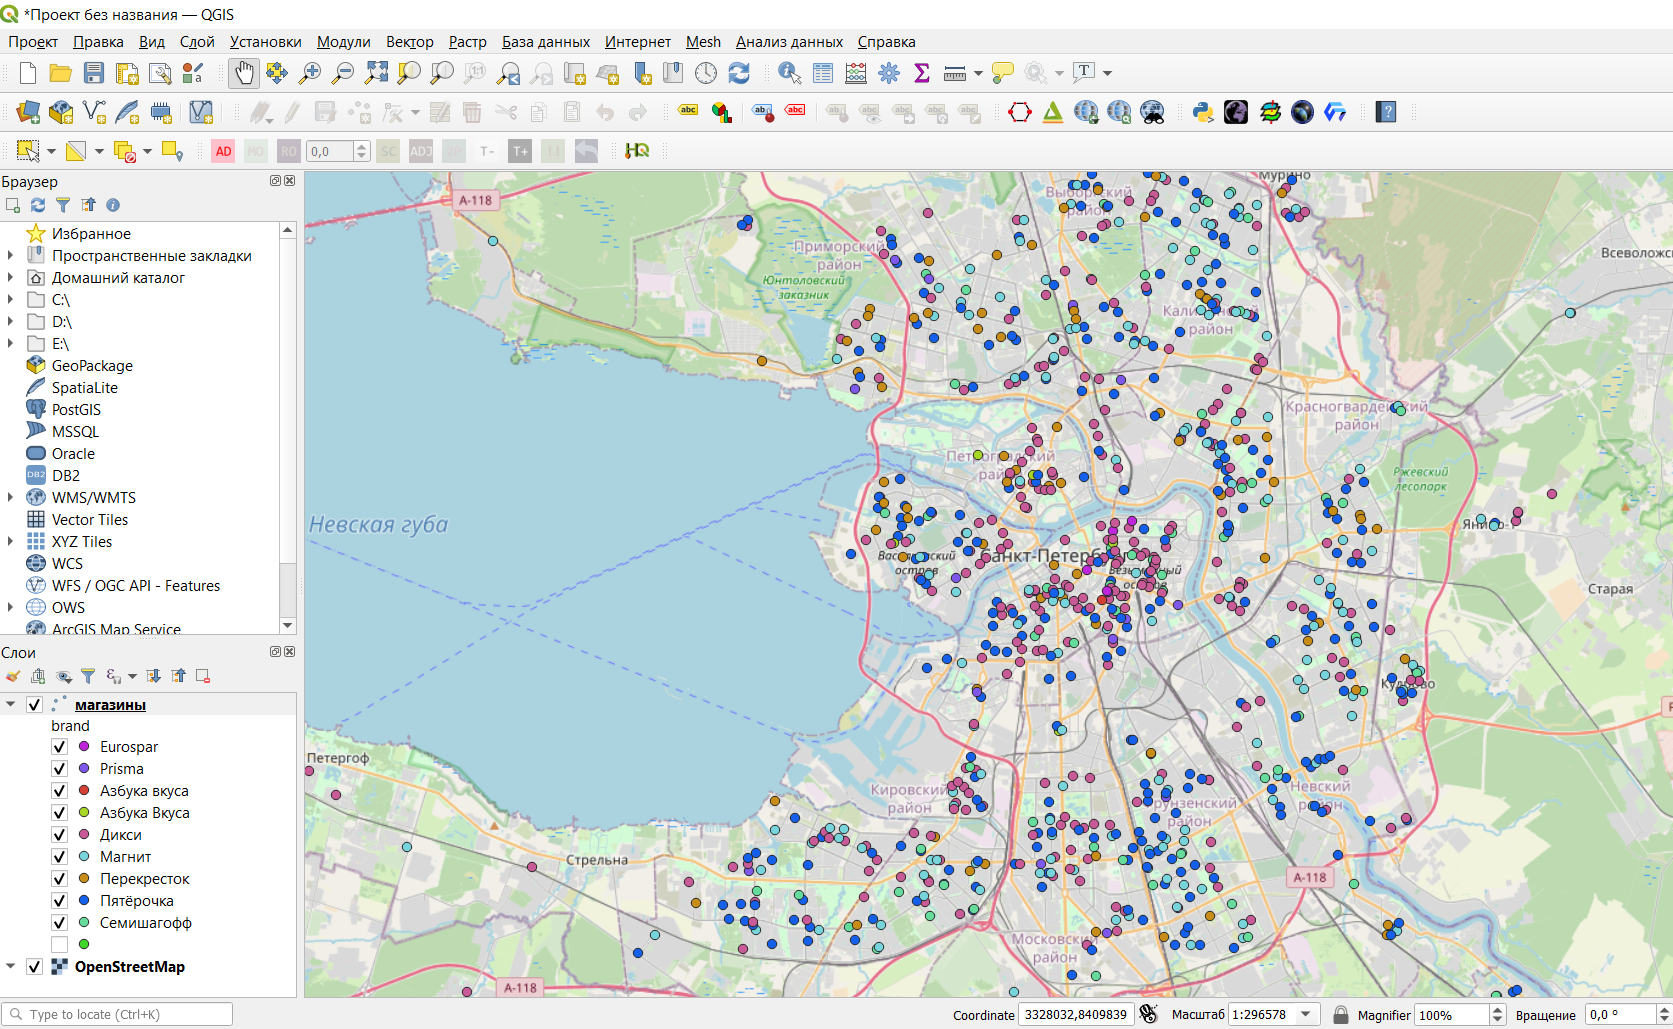
\includegraphics{figures/11.PNG}

Цвета и типы символов можно настраивать дополнительно вручную.\\
Тепловая карта объектов будет выглядеть примерно таким образом, но важно помнить, что она динамически пересчитывается в зависимости от масштаба.

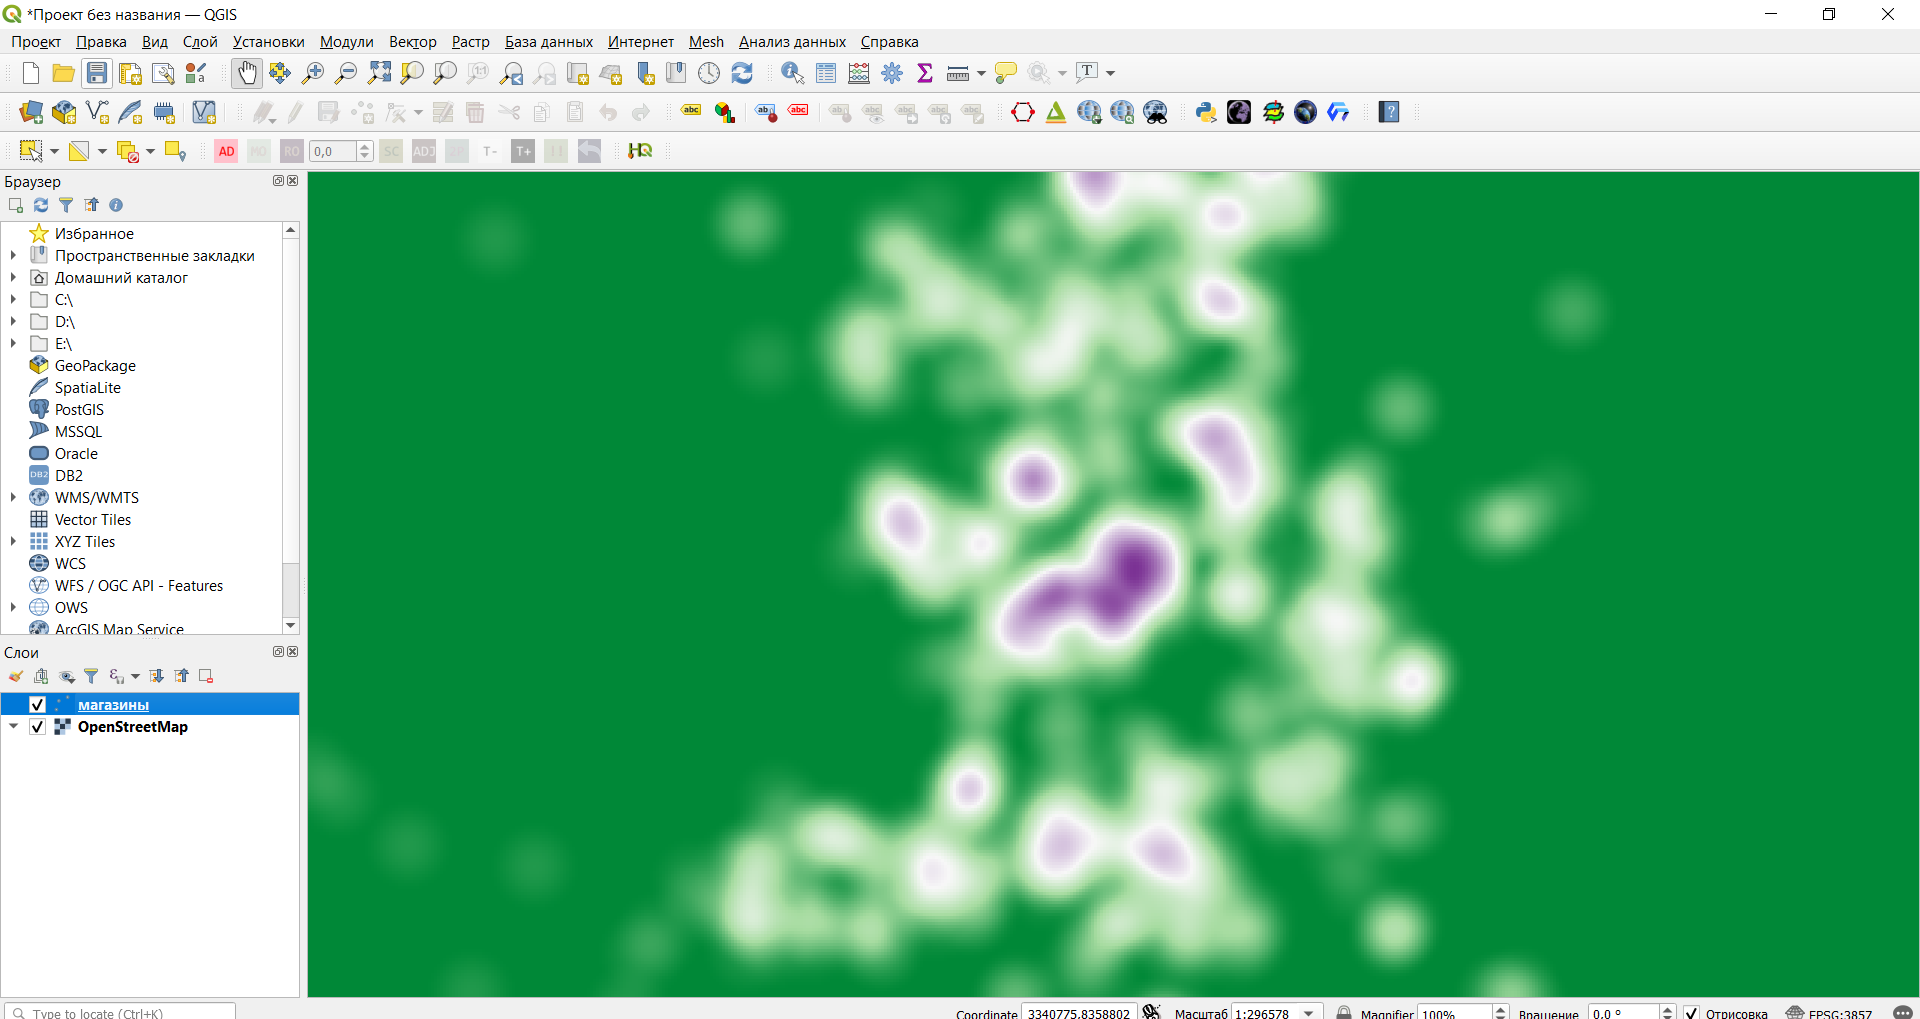
\includegraphics{figures/12.PNG}

В QGIS~описание стиля слоя можно сохранить в формате xml, что позволяет обмениваться стилями оформления ~и применять готовые стили.

Чтобы использовать готовый стиль, нужно скачать файл стиля (например, с ресурса \href{http://qgis-hub.fast-page.org/styles.php}{http://qgis-hub.fast-page.org/styles.php).}.) После~этого нужно выбрать \emph{Управление стилями} в свойствах слоя.

Далее нужно выбрать Импорт/Экспорт→Импорт и выбрать файл с описанием стиля, после чего импортировать его.

\hypertarget{grid}{%
\chapter{Подсчет плотности объектов по сетке}\label{grid}}

\hypertarget{ux43fux43eux441ux442ux440ux43eux435ux43dux438ux435-ux441ux435ux442ux43aux438}{%
\section{Построение сетки}\label{ux43fux43eux441ux442ux440ux43eux435ux43dux438ux435-ux441ux435ux442ux43aux438}}

Построим карту плотности распределения объектов по сетке. Для этого нужно будет сначала включить панель инструментов анализа либо через строку меню \textbf{Вид ⤑Панели⤑ Инструменты анализа}, либо \textbf{Анализ данных ⤑Панель инструментов}.

Панель должна появиться в правой части окна программы.

Для начала создадим сетку с помощью инструмента \emph{Create grid}.

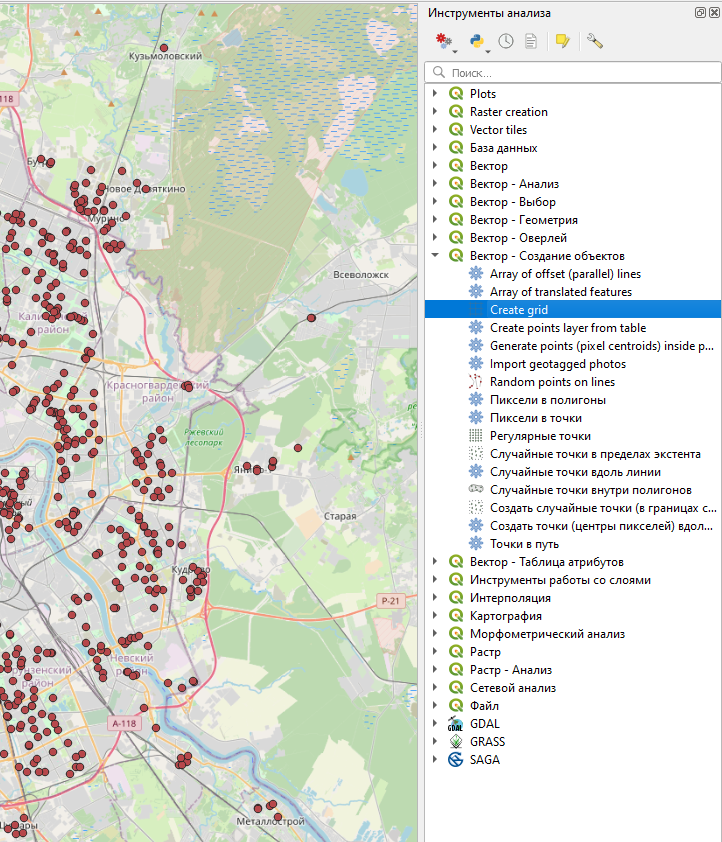
\includegraphics{figures/13.png}

После этого нужно задать параметры сетки.

Сетка может быть создана в виде точек, линий, прямоугольников, шестиугольников и ромбов. Наиболее распространено применение прямоугольной/квадратной сетки и сетки правильный шестиугольников.

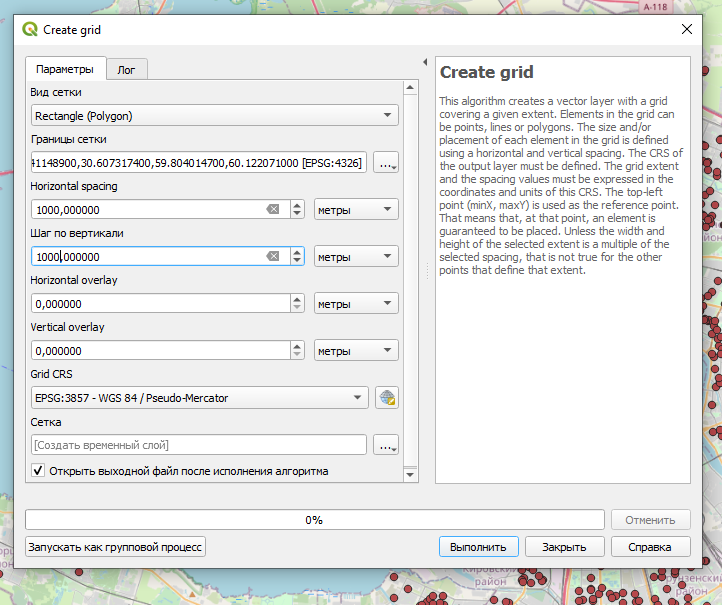
\includegraphics{figures/14.png}

Границы сетки лучше делать по границам того, слоя, который будет впоследствии агрегироваться по этой сетке.

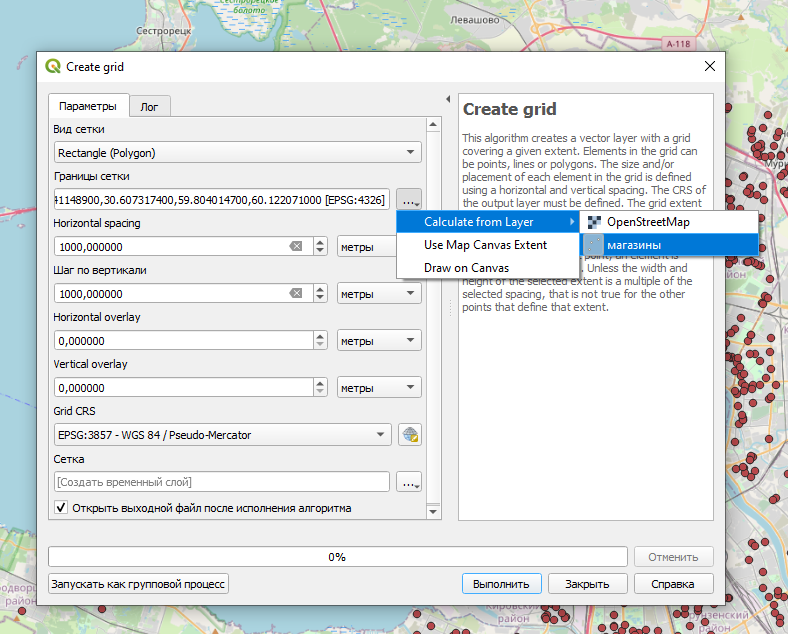
\includegraphics{figures/15.png}

\begin{quote}
Важно помнить, что выбор размера ячейки сетки является очень важным: если ячейки будут слишком большие, то данные будут чересчур обобщенными, если ячейки будут слишком маленькими, то результат получится слишком дробным.
\end{quote}

\begin{quote}
Также следует помнить, что если вы не сохраните временные файлы, полученные в результате выполнения операции, они будут существовать только в течение текущего сеанса работы. Файлы можно сохранять сразу при задании параметров операции, либо после с помощью команды Экспорт или Сохранить на диск контекстного меню слоя.
\end{quote}

В результате будет получена сетка квадратов

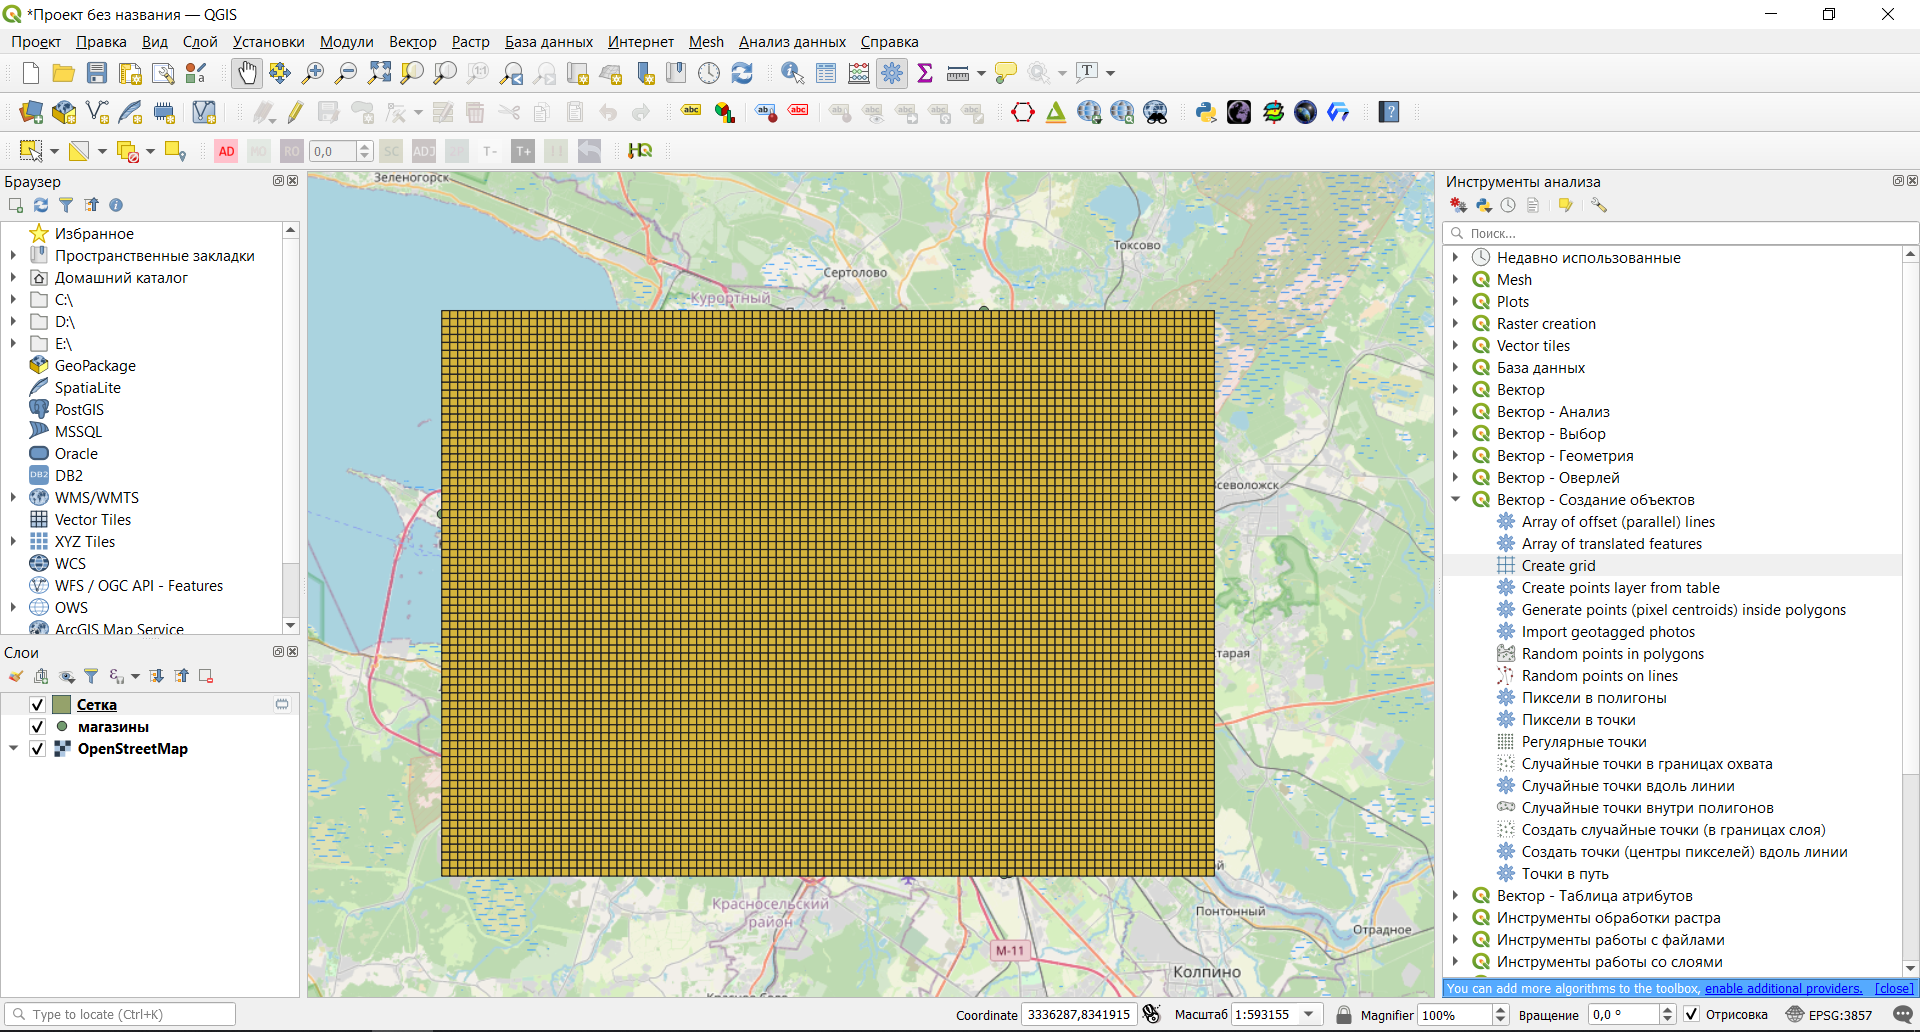
\includegraphics{figures/16.PNG}

\hypertarget{ux43fux43eux434ux441ux447ux435ux442-ux43aux43eux43bux438ux447ux435ux441ux442ux432ux430-ux43eux431ux44aux435ux43aux442ux43eux432}{%
\section{Подсчет количества объектов}\label{ux43fux43eux434ux441ux447ux435ux442-ux43aux43eux43bux438ux447ux435ux441ux442ux432ux430-ux43eux431ux44aux435ux43aux442ux43eux432}}

Для того, чтобы посчитать число объектов, попадающих в каждую ячейку сетки, нужно воспользоваться функцией \emph{Пространственное соединение (summary)}.

Операция пространтсвенного соединения необходима для того, чтобы присоединить атрибуты объектов одного слоя к объектам другого слоя с учетом взаимного расположения объектов. Например, присвоить адреса домов объектам, расположенным внутри этих домов.

\emph{Пространственное соединение (summary) (}в более новых версиях может называться \emph{Присоединить атрибуты по пространственному положению (сводка)})не просто присоединяет атрибуты, но еще и подсчитывает статистические показатели по исходным атрибутам.

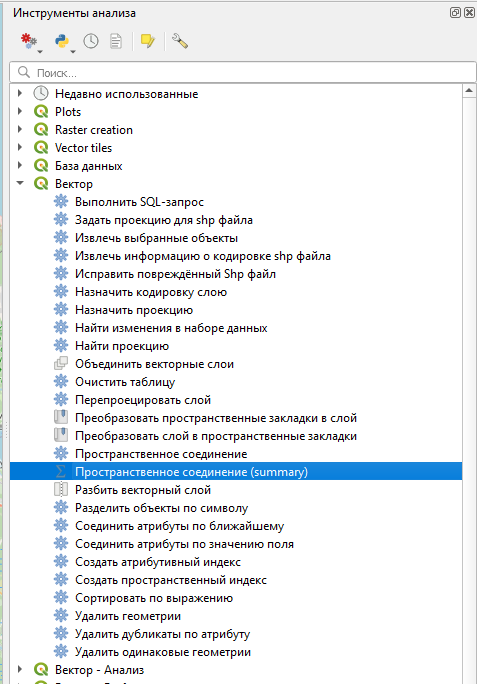
\includegraphics{figures/17.png}

Сначала нужно выбрать исходный слой (тот слой, которому будем приписывать новые атрибуты) и связанный слой (из которого эти атрибуты будут извлекаться), а также геометрический предикат (как объекты разных слоев расположены относительно друг друга).

В нашем случае в качестве геометрического предиката выступает \emph{contains}, потому что ячейки сетки содержат в себе точки с магазинами.

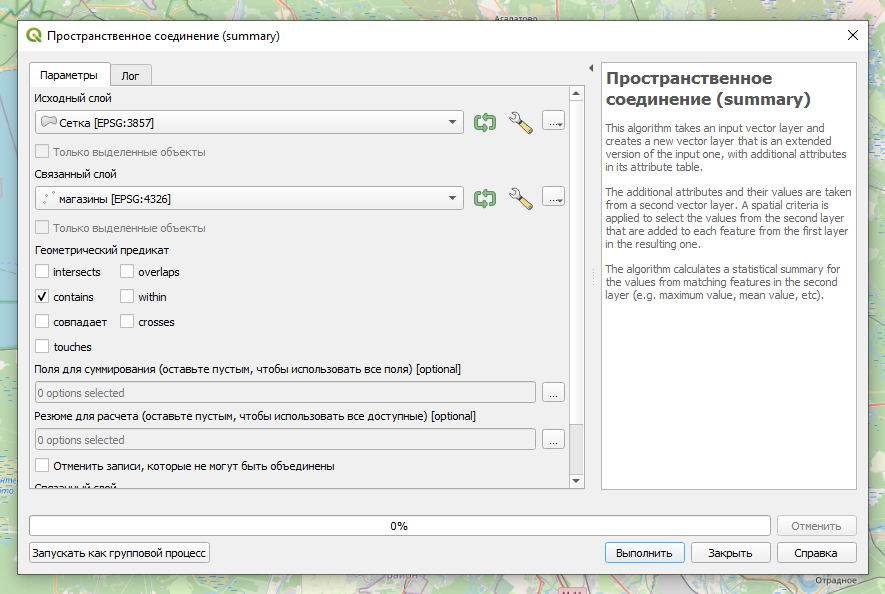
\includegraphics{figures/18.png}

Далее выбираем поля для суммирования. Если не будет выбрано ни одно поле, то будут взяты все атрибуты из связанного слоя. В нашем случае нам достаточно будет атрибута \emph{brand}.

Далее выбираем резюме для расчета. Если не указать конкретный тип показателя, то программа будет рассчитывать все возможные показатели. Так как мы рассчитываем количество точек, то резюме для расчета нужно выбрать \emph{count}.

Параметр \emph{Отменить записи, которые не могут быть объединены}~позволяет удалить те объекты исходного слоя, к которым не нашлось подходящих объектов связанного слоя.

Связанный слой лучше сохранить в файл.

Результат соединения (с включенным параметром \emph{Отменить записи, которые не могут быть объединены}).

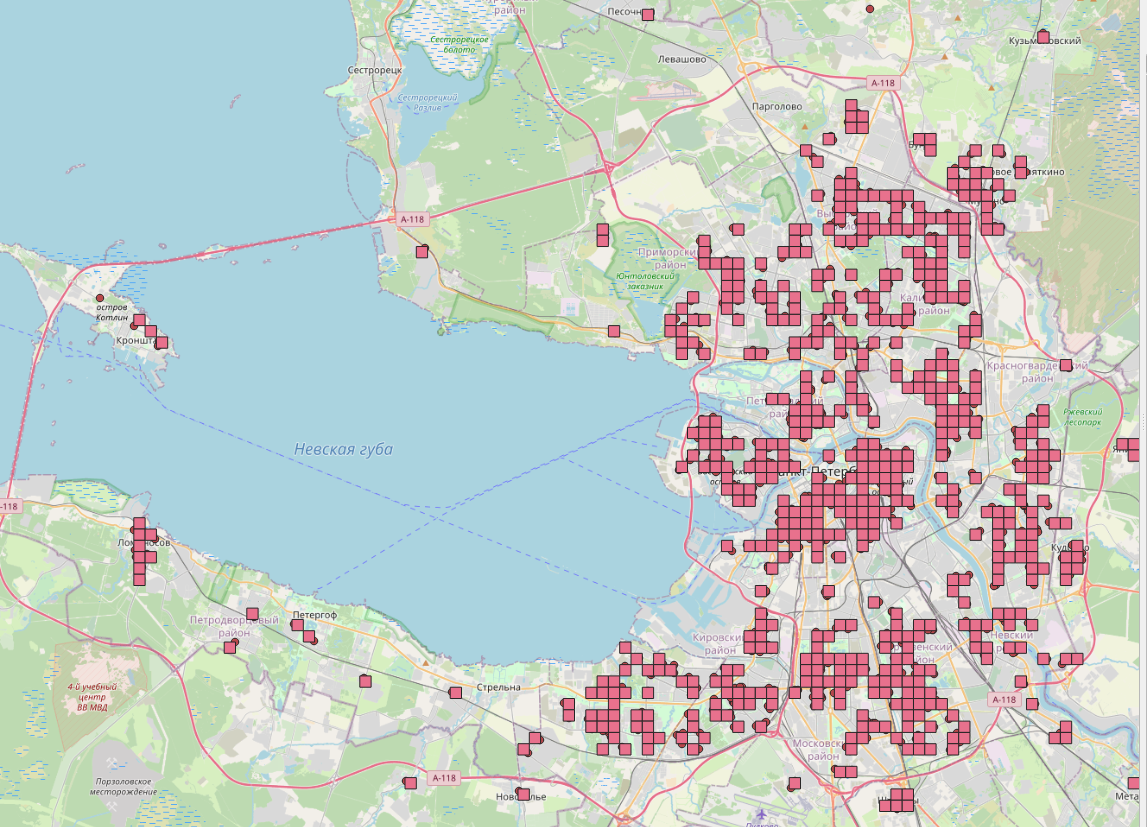
\includegraphics{figures/19.png}

Таблица атрибутов полученного слоя

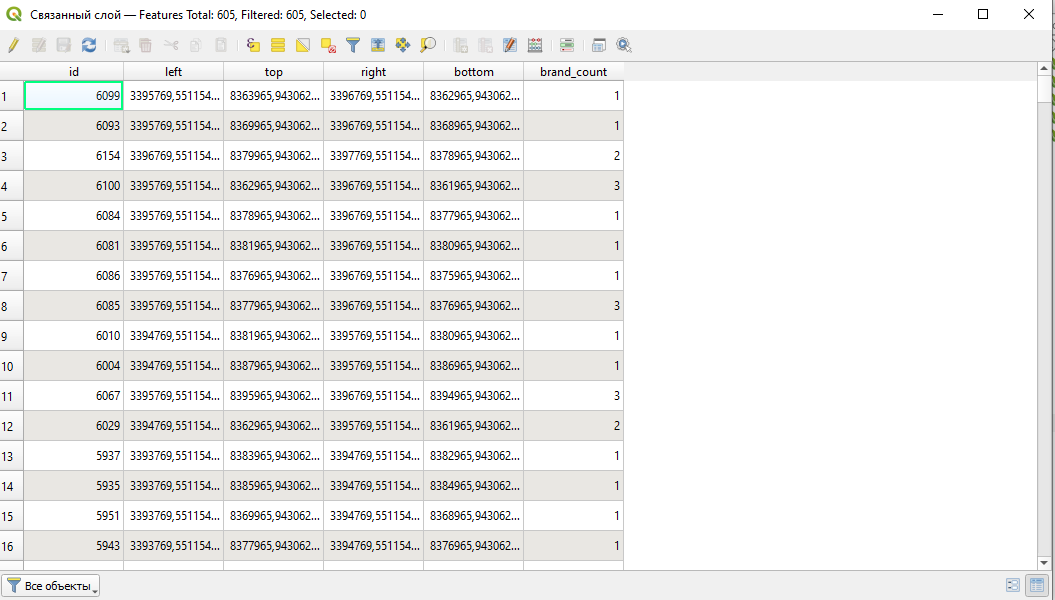
\includegraphics{figures/20.png}

Поля \emph{id, left, top, right, bottom} были созданы при изначальном построении сетки, а в поле \emph{brand\_count} у нас содержится посчитанное число точек, попадающих в соотвествующую ячейку.

Далее мы можем настроить цвет ячейки в зависимости от числа точек.

Для этого в настройках стиля слоя нужно выбрать \textbf{\emph{Градуированный знак}}, потом Значение по колонке \emph{brand\_count}.

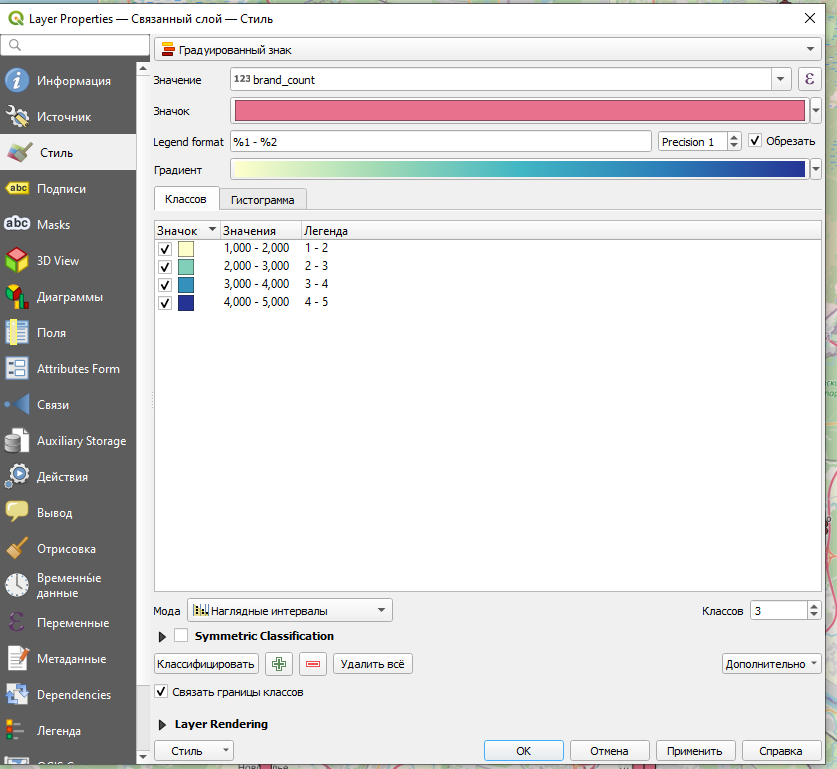
\includegraphics{figures/21.png}

Градиент можно выбрать из предложенных имеющихся или создать самостоятельно.

Для того, чтобы появилось разделение объектов не группы, нужно нажать кнопку \emph{Классифицировать}.

Для классификации можно менять тип разбивки на группы (\emph{Мода}) и число классов. Самые широко применяемые методы классификации -- \emph{естественные интервалы Natural breaks}~(создают группы так, чтобы разница между ними была максимальной), \emph{равные интервалы}~(весь интервал изменения показателя делится на равные отрезки) и \emph{равное количество (квантиль)}~(при этом типе классификации во всех группах будет одинаковое количество объектов).

Чтобы лучше понять, как осуществилась разбивка на группы, можно перейти во вкладку \emph{Гистограмма}~и нажать \emph{Load values}. После этого будет построен график распределения объектов ~по величине показателя и показана разбивка на группы.

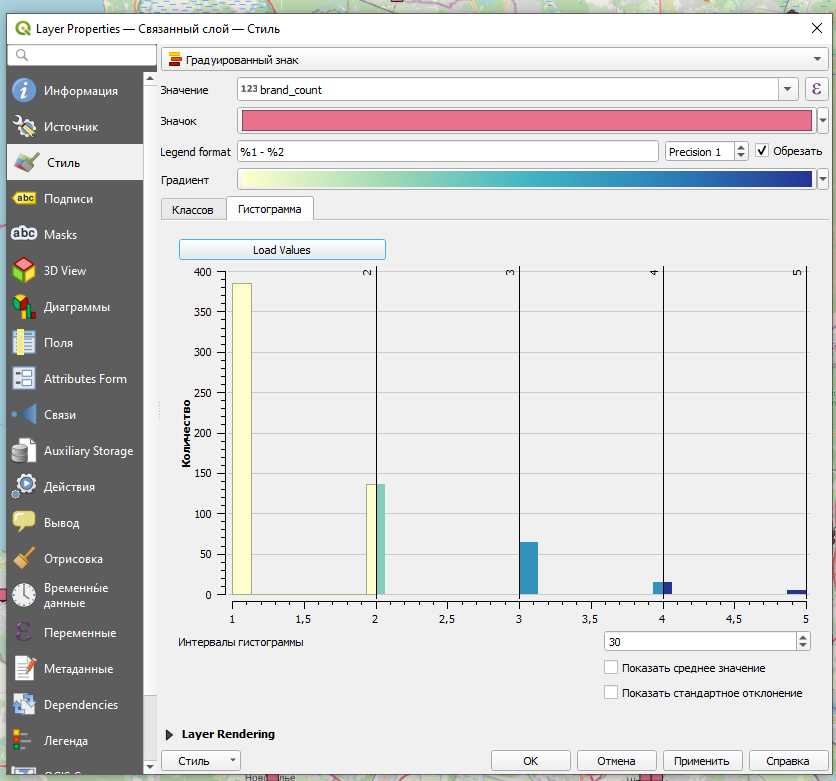
\includegraphics{figures/22.png}

Полученная в результате карта

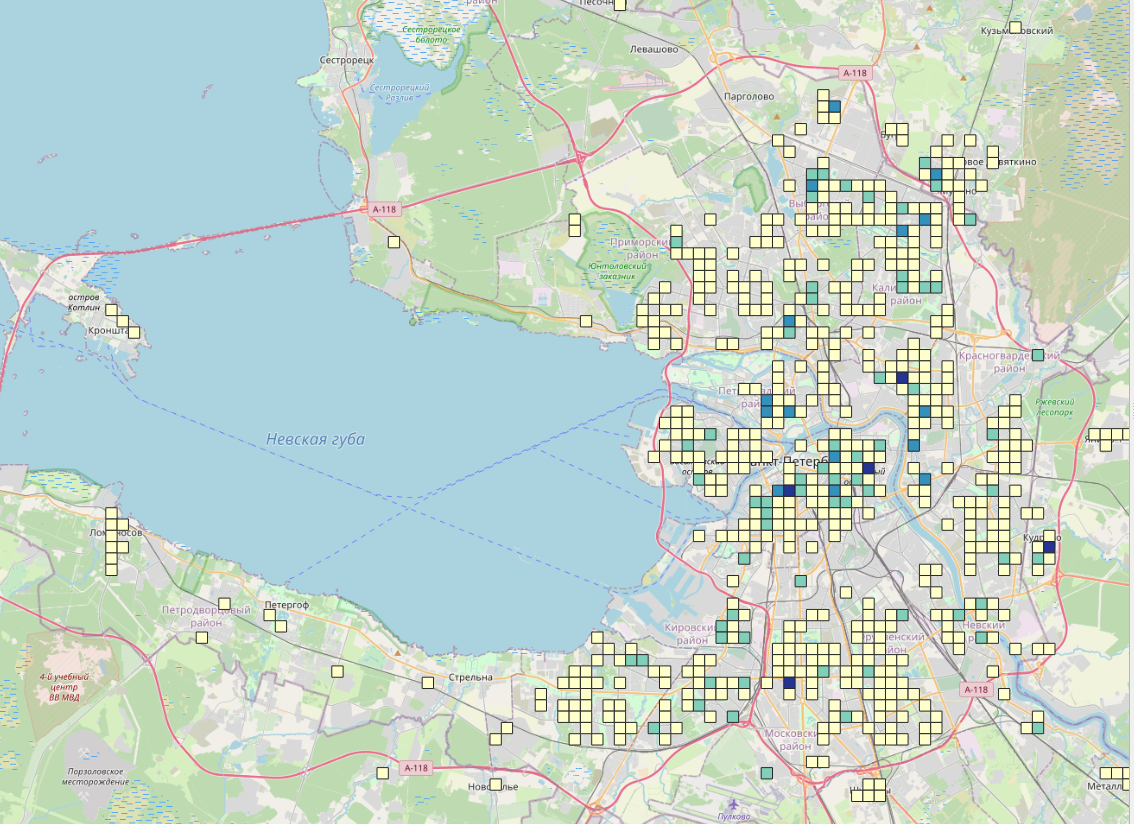
\includegraphics{figures/23.png}

\hypertarget{ux441ux442ux438ux43bux438ux437ux430ux446ux438ux44f-ux441ux43bux43eux44f}{%
\section{Стилизация слоя}\label{ux441ux442ux438ux43bux438ux437ux430ux446ux438ux44f-ux441ux43bux43eux44f}}

Полученную карту мы стилизовали \emph{«в стиле Lego»}.

Чтобы это сделать сначала нужно построить центроиды для квадратов сетки (функция \emph{Центроиды}~в панели инструментов анализа), потом этим центроидам задать те же самые настройки цвета, что и квадратам сетки.

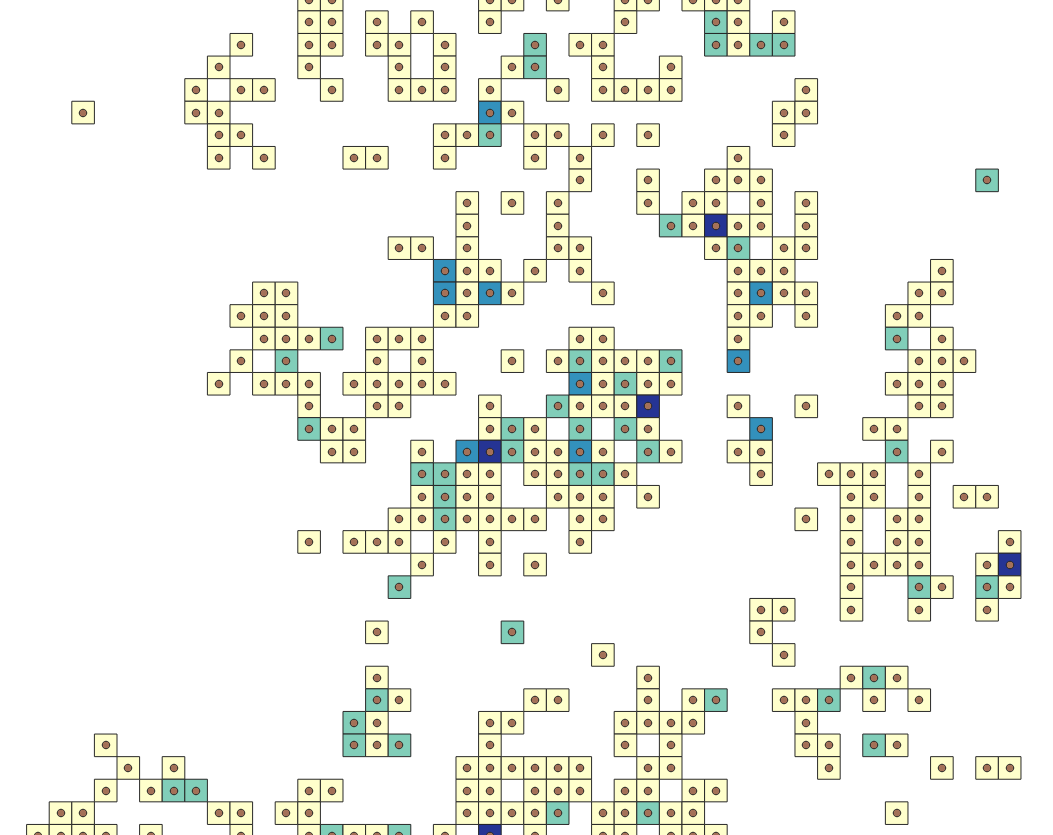
\includegraphics{figures/24.png}

Настроим цвета и размеры символов

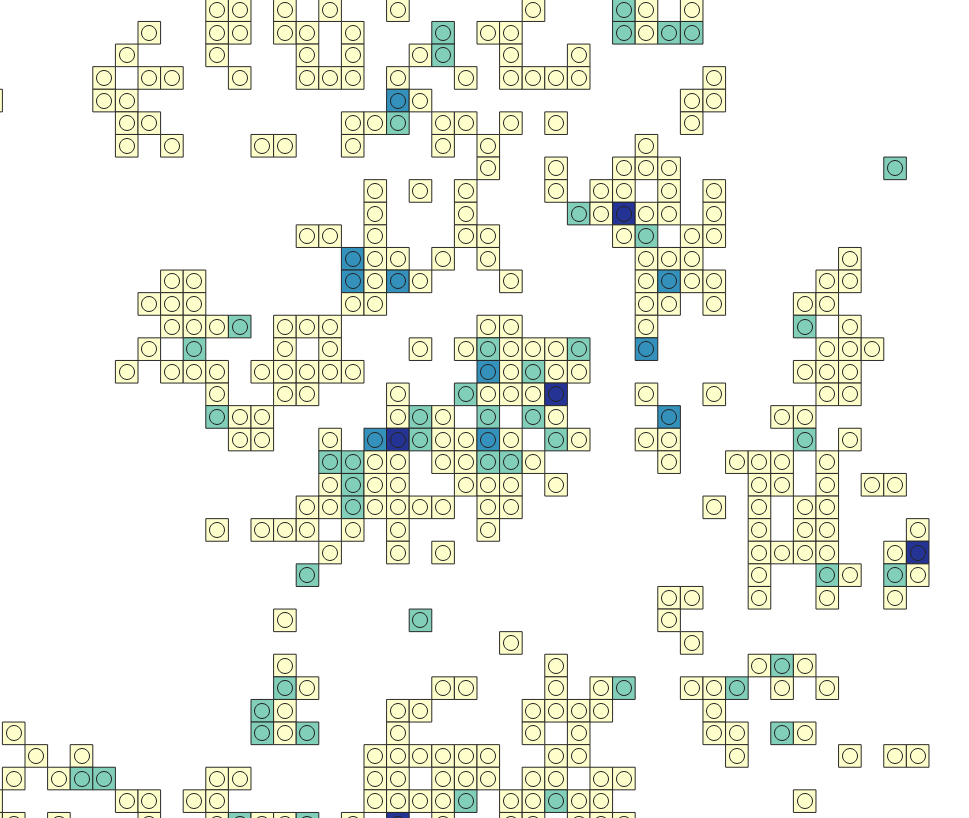
\includegraphics{figures/25.png}

Добавим ``тень''. Для этого нужно продублировать слой центроидов, сделать их черного или темно-серого цвета и настроить небольшое смещение.

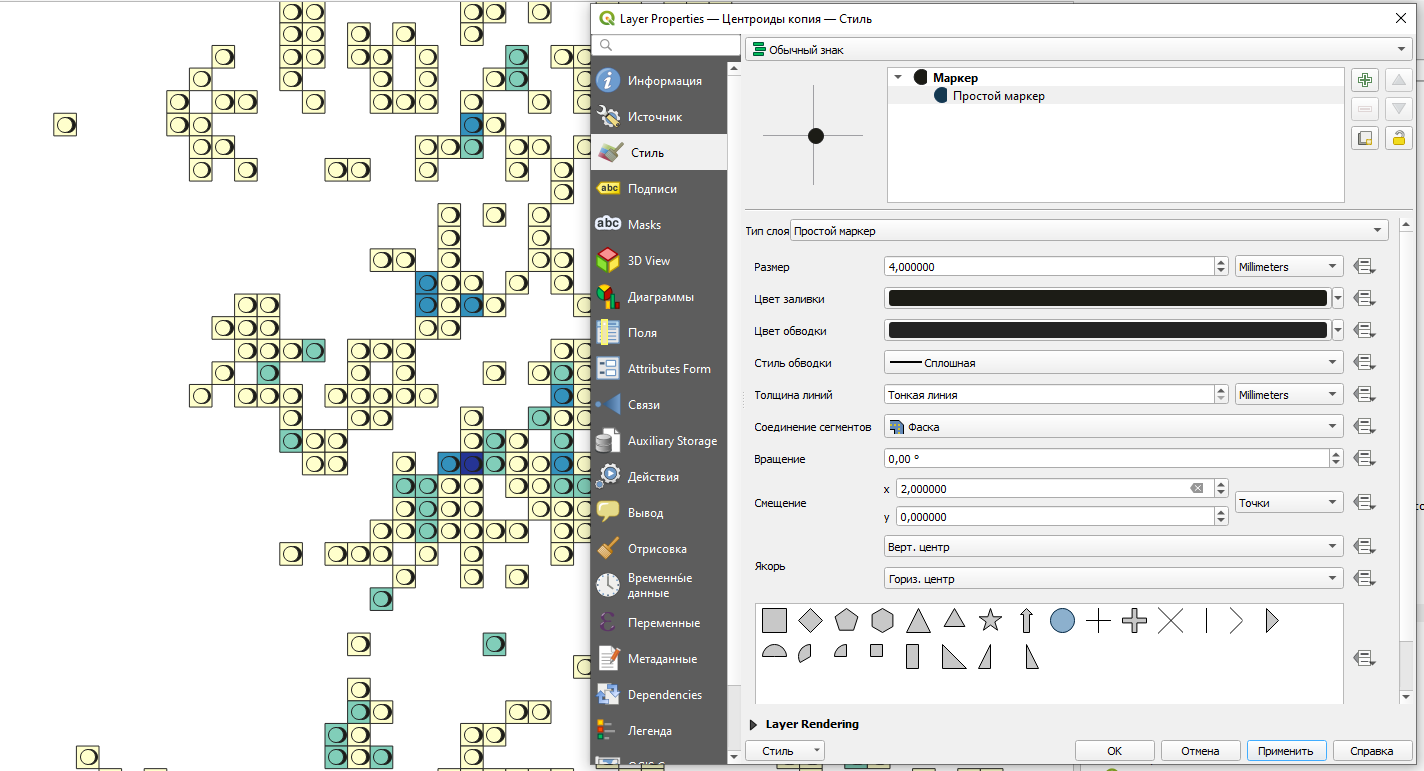
\includegraphics{figures/26.png}

\hypertarget{ux43eux444ux43eux440ux43cux43bux435ux43dux438ux435-ux43aux430ux440ux442ux44b}{%
\section{Оформление карты}\label{ux43eux444ux43eux440ux43cux43bux435ux43dux438ux435-ux43aux430ux440ux442ux44b}}

Для того, чтобы оформить карту для печати, отчета или документации используют макеты. Макеты являются частью проекта.

Создание макета осуществляется из строки меню \textbf{Проект⤑Создать макет}. Имя макета можно задать самостоятельно или оно будет задано автоматически по умолчанию.

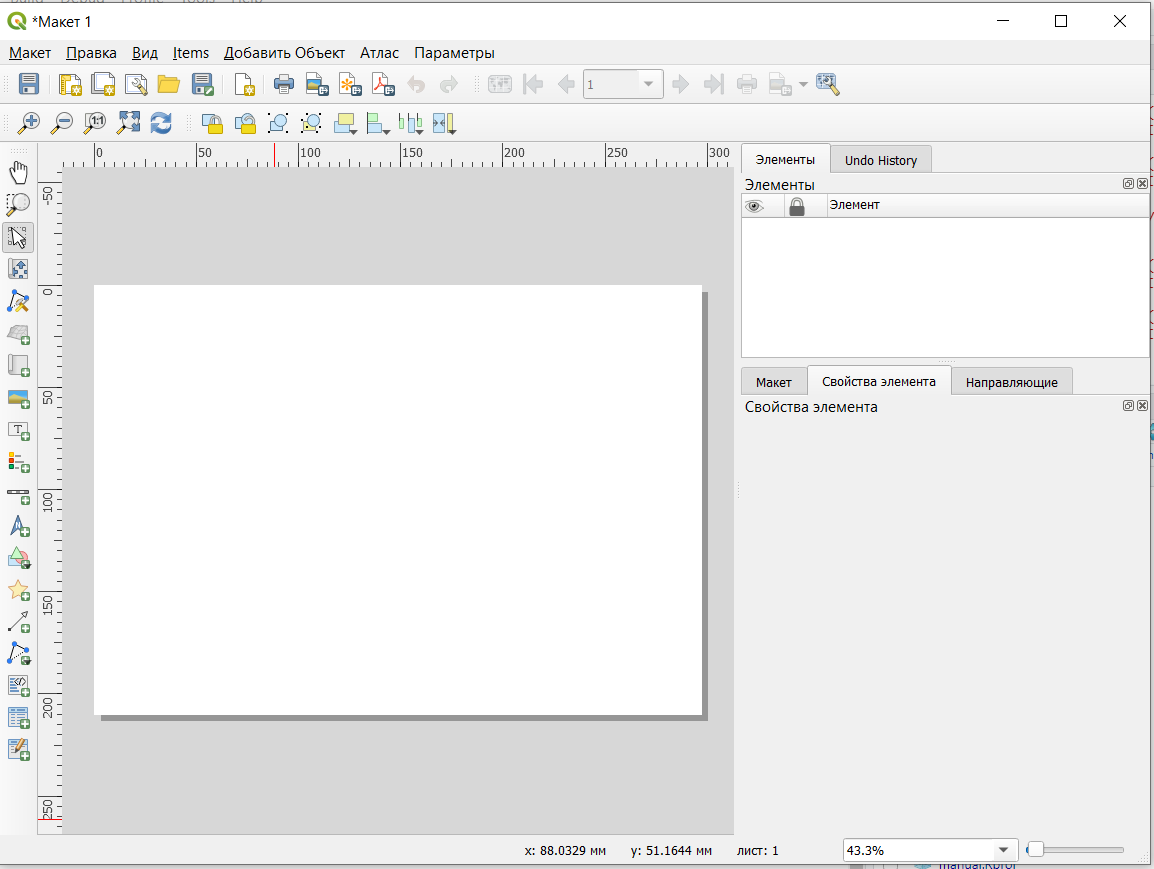
\includegraphics{figures/27.PNG}

По умолчанию макет создается на листе формата А4 в альбомной ориентации, формат и ориентацию листа можно заменить в параметрах листа.

Слева в окне создания макета расположена панель добавления элементов, справа - перечень элементов и настройки конкретных элементов.

Для того, чтобы добавить на макет карту, нужно выбрать инструмент \emph{Добавить карта}, щелкнуть на участок на листе, куда карту нужно добавить. В карте отображаются те же слои, которые являются видимыми в проекте, при отключении/включении слоев изображение на макете будет меняться. Чтобы этого не происходило, нужно заблокировать слои в настройках элемента карты.

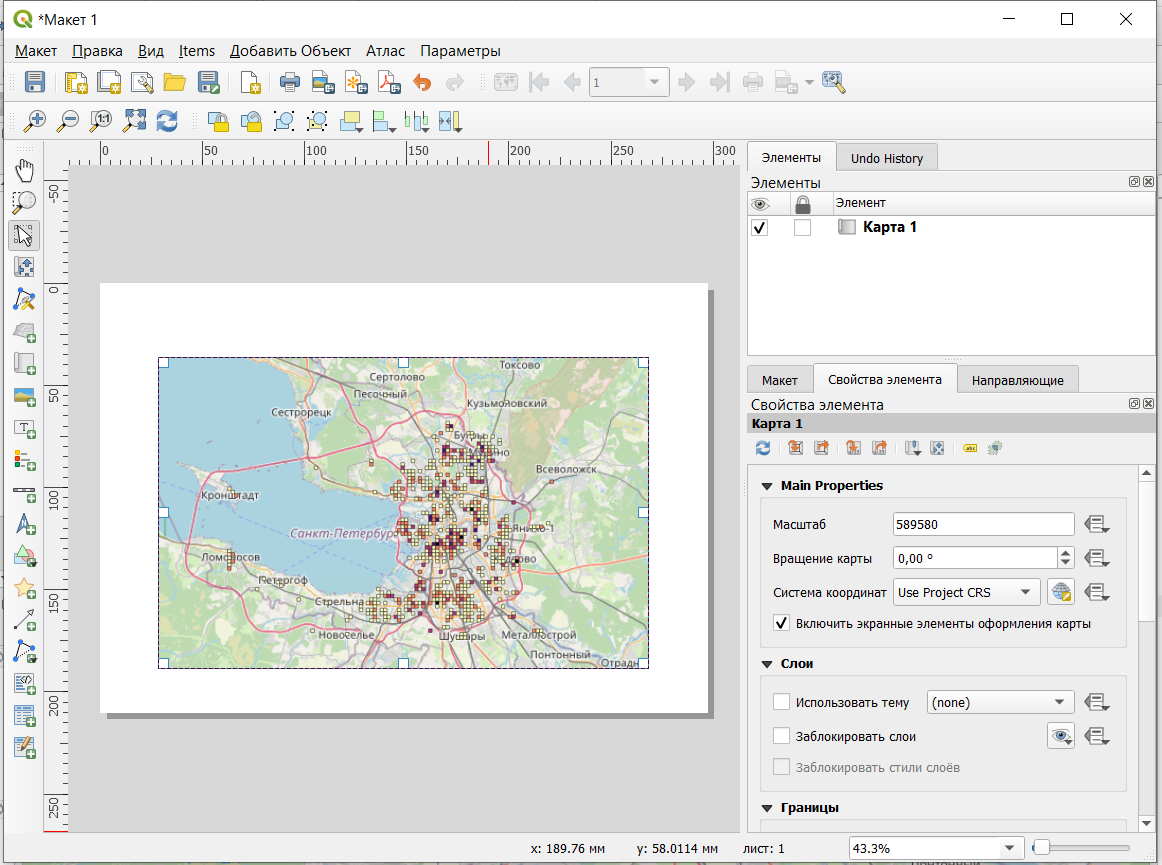
\includegraphics{figures/28.PNG}

Для карты можно настроить нужный масштаб, угол поворота при необходимости и систему координат.

Другими важными элементами оформления карты являются масштабная линейка и легенда. Эти элементы добавляются соответствующими кнопками на панели добавления элементов и далее настраиваются по необходимости.

В масштабной линейке может быть настроен тип линейки, размер и число отрезков на линейке. Важно помнить, ч то размер отрезков может быть задан как в единицах измерения карты (\emph{Фиксированная ширина}), так и в единицах измерения листа (\emph{Зафиксировать длину сегмента}).

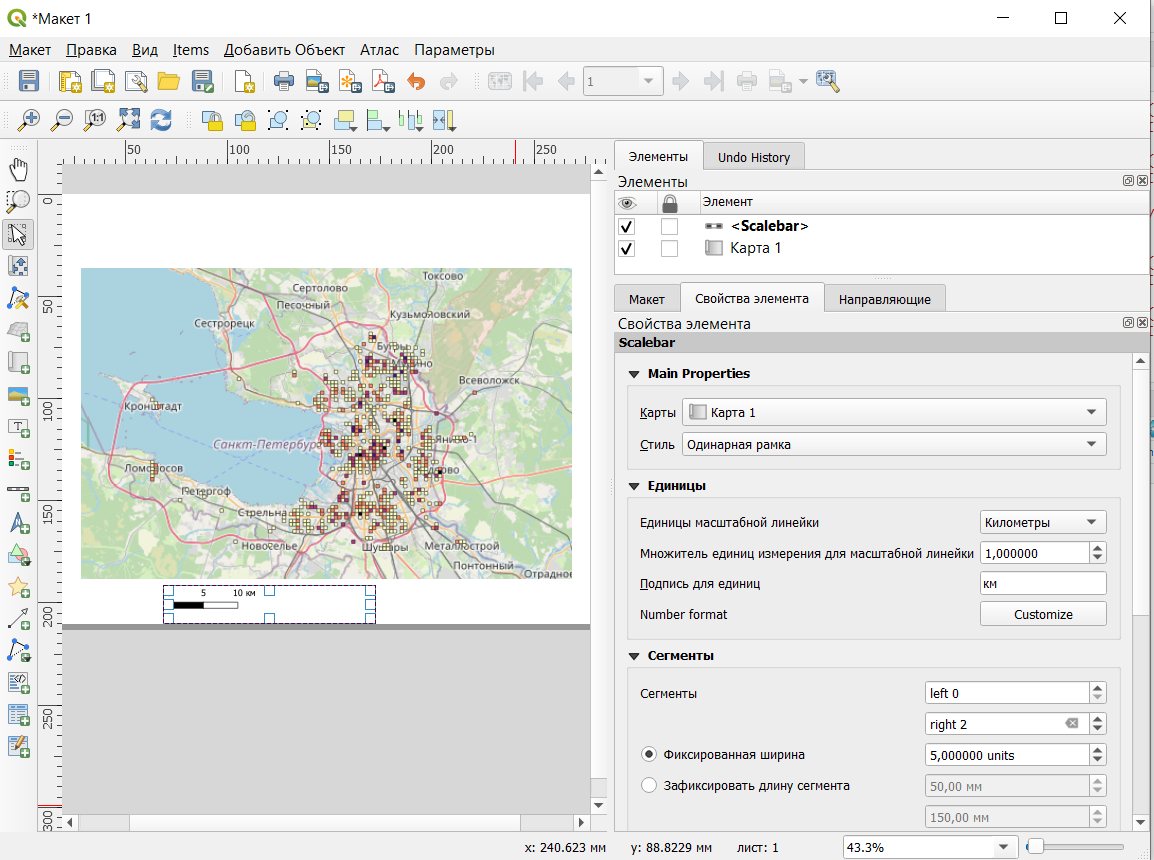
\includegraphics{figures/29.PNG}

Легенда добавляется по умолчанию с полным перечнем слоев проекта и с теми же названиями как в проекте.

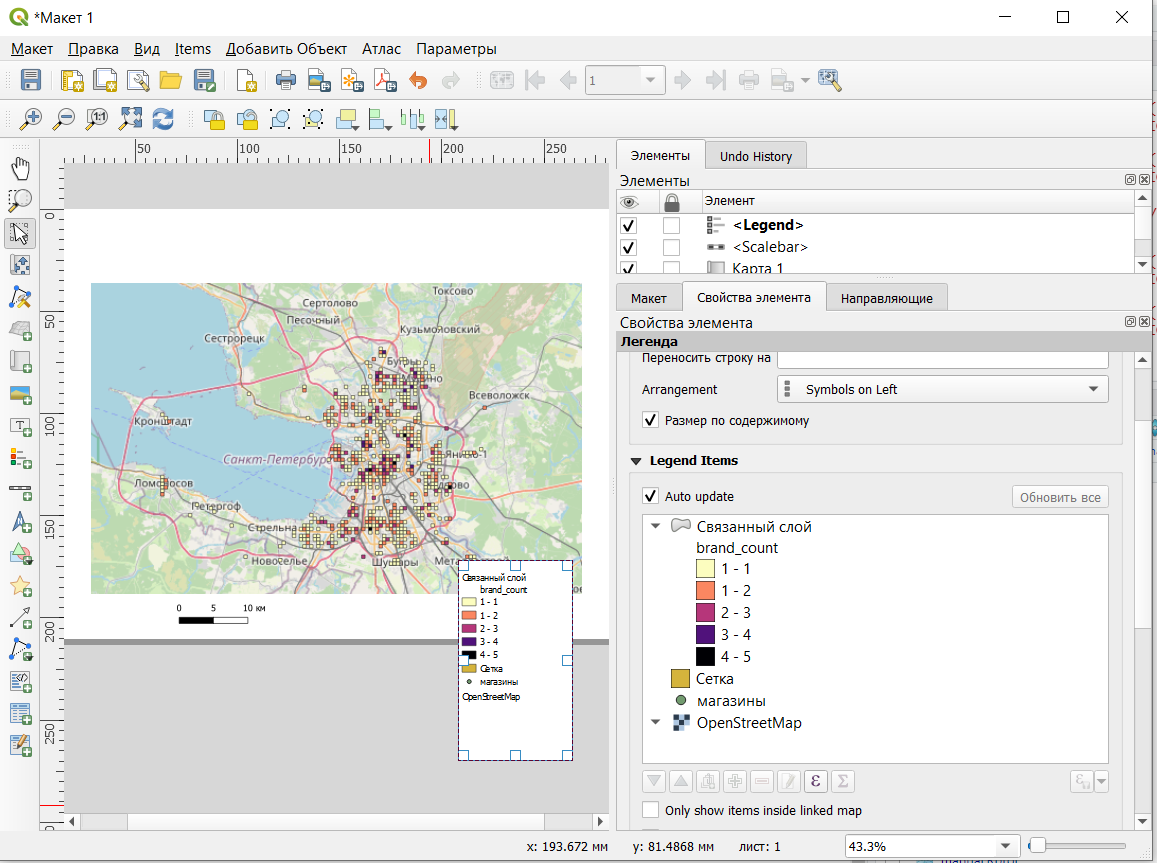
\includegraphics{figures/30.PNG}

При необходимости можно отключить автоматическое обновление легенды и скорректировать названия слоев и их перечень в легенде.

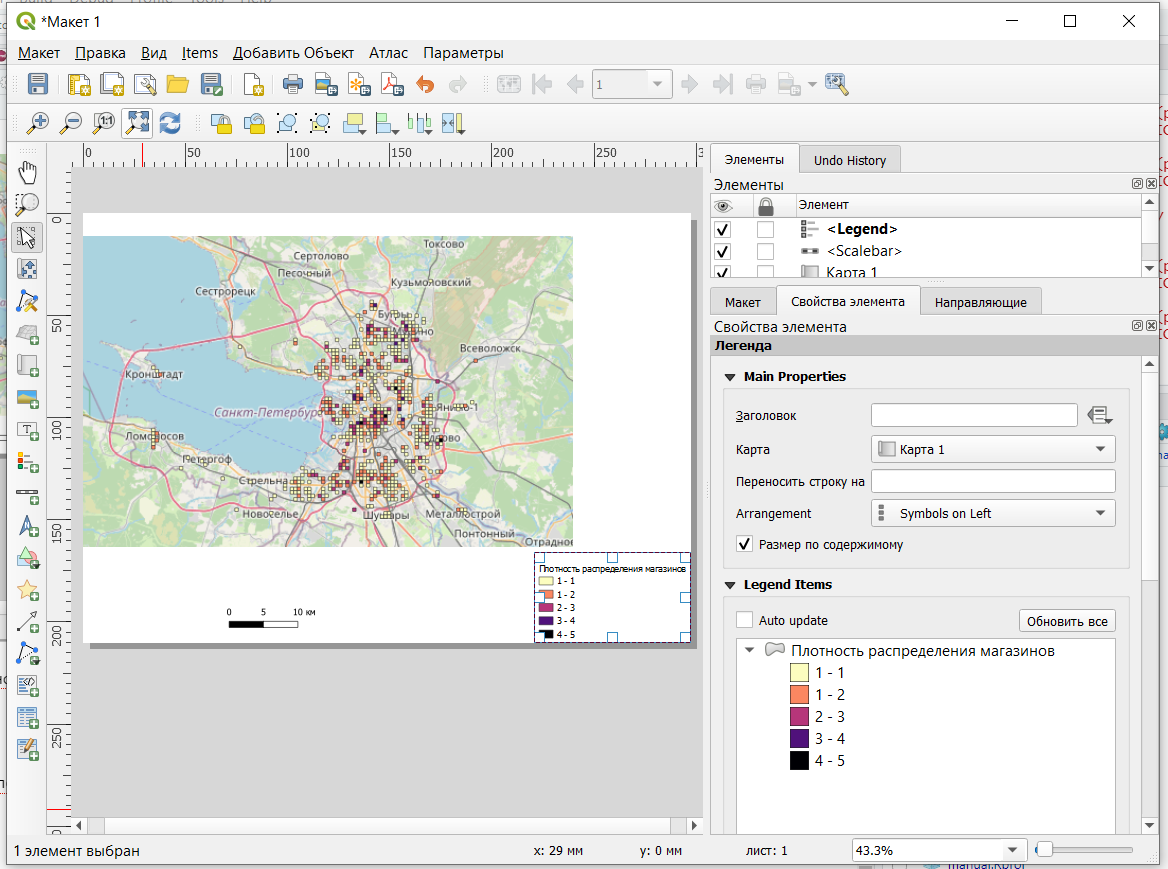
\includegraphics{figures/31.PNG}

Готовую карту можно экспортировать для печати в формат изображения или pdf.

\hypertarget{ux437ux430ux433ux440ux443ux437ux43aux430-ux434ux430ux43dux43dux44bux445-ux447ux435ux440ux435ux437-ux441ux435ux440ux432ux438ux441-overpass-turbo}{%
\chapter{Загрузка данных через сервис overpass-turbo}\label{ux437ux430ux433ux440ux443ux437ux43aux430-ux434ux430ux43dux43dux44bux445-ux447ux435ux440ux435ux437-ux441ux435ux440ux432ux438ux441-overpass-turbo}}

\textbf{OpenStreetMap (OSM)} --- проект, который создаёт и предоставляет свободные географические данные, дает возможность создавать карты любому пользователю. Каждый желающий может поучаствовать в проекте (загружать свои треки на сервер, дорисовывать общедоступную карту по спутниковым снимкам Bing, MapBox, DigitalGlobe (весь мир), IRS (запад России), SPOT4 (восток России) и SPOT (Белоруссия) от Космоснимки.ру, ASTER (Россия), OrbView-3 и другими) и использовать эти карты совершенно свободно, и бесплатно в отличие от многих других карт, даже бесплатных, свободное использование которых ограничено.

Карты этого проекта очень широко используются как в некоммерческих целях, например, для исследовательских проектов, так и для коммерческих проектов, например, создания навигационных приложений. Один из самых простых способов скачивания пространственных данных с OSM - это использование сервиса \url{http://overpass-turbo.eu/}.

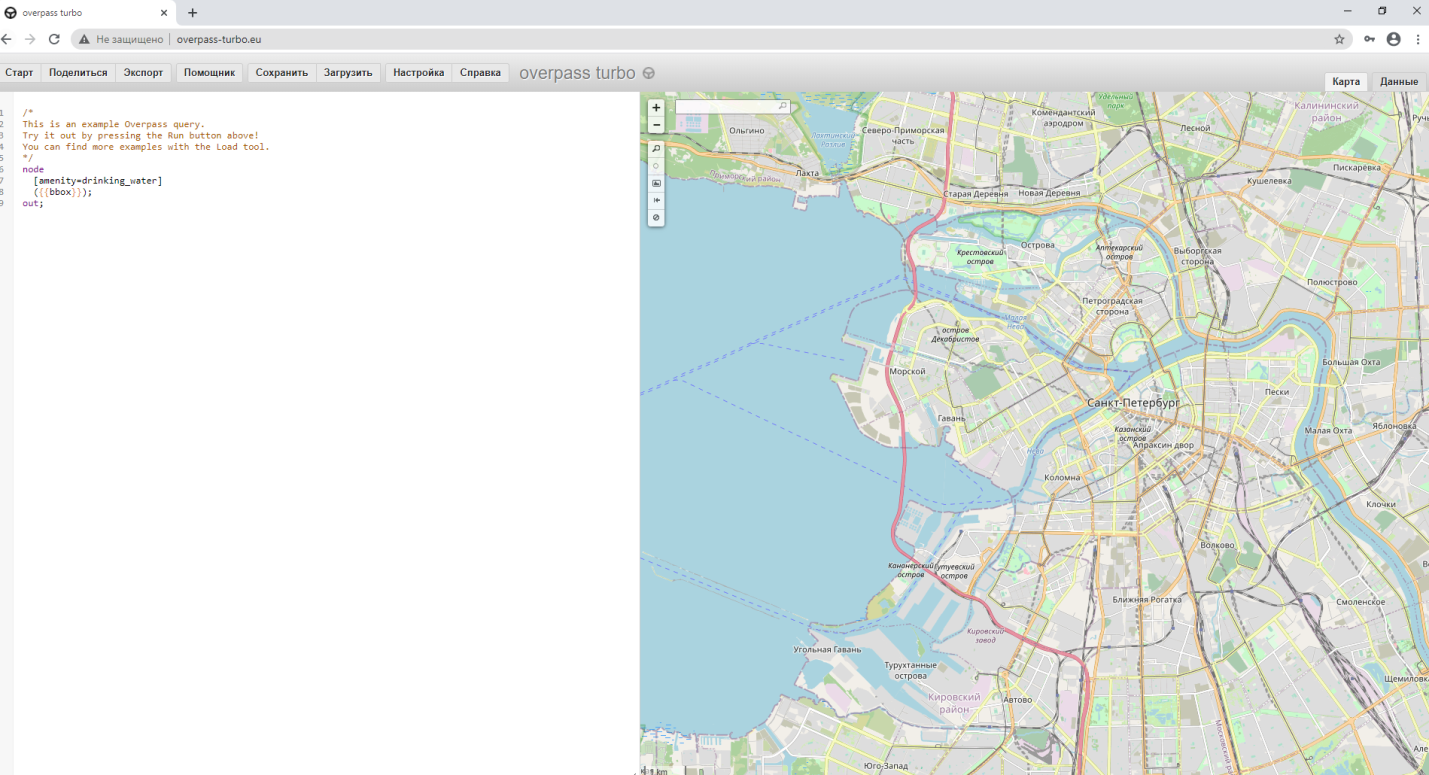
\includegraphics{figures/32.png}

Подробная информация о сервисе \href{https://wiki.openstreetmap.org/wiki/Overpass_turbo}{\underline{https://wiki.openstreetmap.org/wiki/Overpass\_turbo}}

Подробная информация о том, какие объекты как \href{https://wiki.openstreetmap.org/wiki/RU:\%D0\%9E\%D0\%B1\%D1\%8A\%D0\%B5\%D0\%BA\%D1\%82\%D1\%8B_\%D0\%BA\%D0\%B0\%D1\%80\%D1\%82\%D1\%8B}{обозначаются в OpenStreetMap}

В левой части окна будет отображаться выполняемый запрос, а в правой результаты этого запроса. По умолчанию поиск осуществляется в той области, которая отображается в правой части окна (это можно скорректировать более сложными запросами, см. справку о сервисе).

Для составления запросов используется помощник

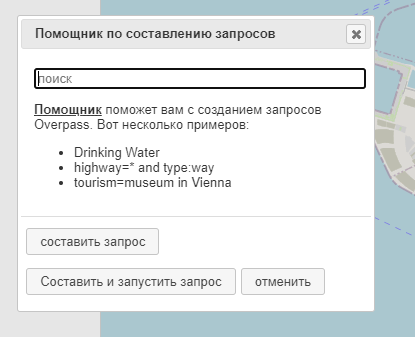
\includegraphics{figures/33.png}

Мы производили поиск жилых зданий, они ищутся по запросу \emph{building=residential}. Поиск осуществляется в той области, которая видна в правой части окна, поэтому перед выполнением запроса нужно найти нужную часть города (можно взять один район или несколько кварталов Санкт-Петербурга).

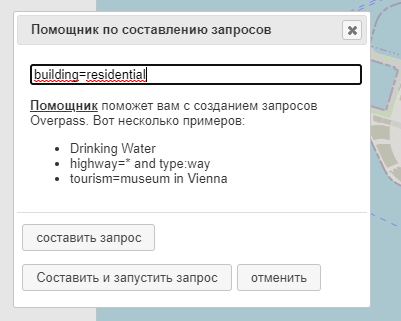
\includegraphics{figures/34.png}

Запрос у вас должен получиться примерно такой (строчку, начинающуюся с node можно убрать вручную)

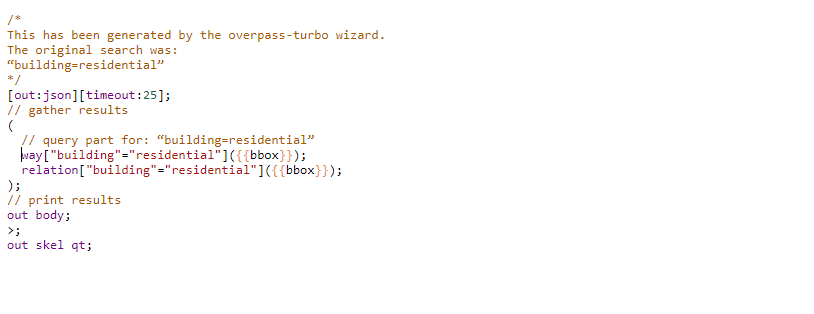
\includegraphics{figures/35.png}

После нажатия кнопки \emph{Старт}~запрос будет выполнен и результаты отобразятся в правой части окна.

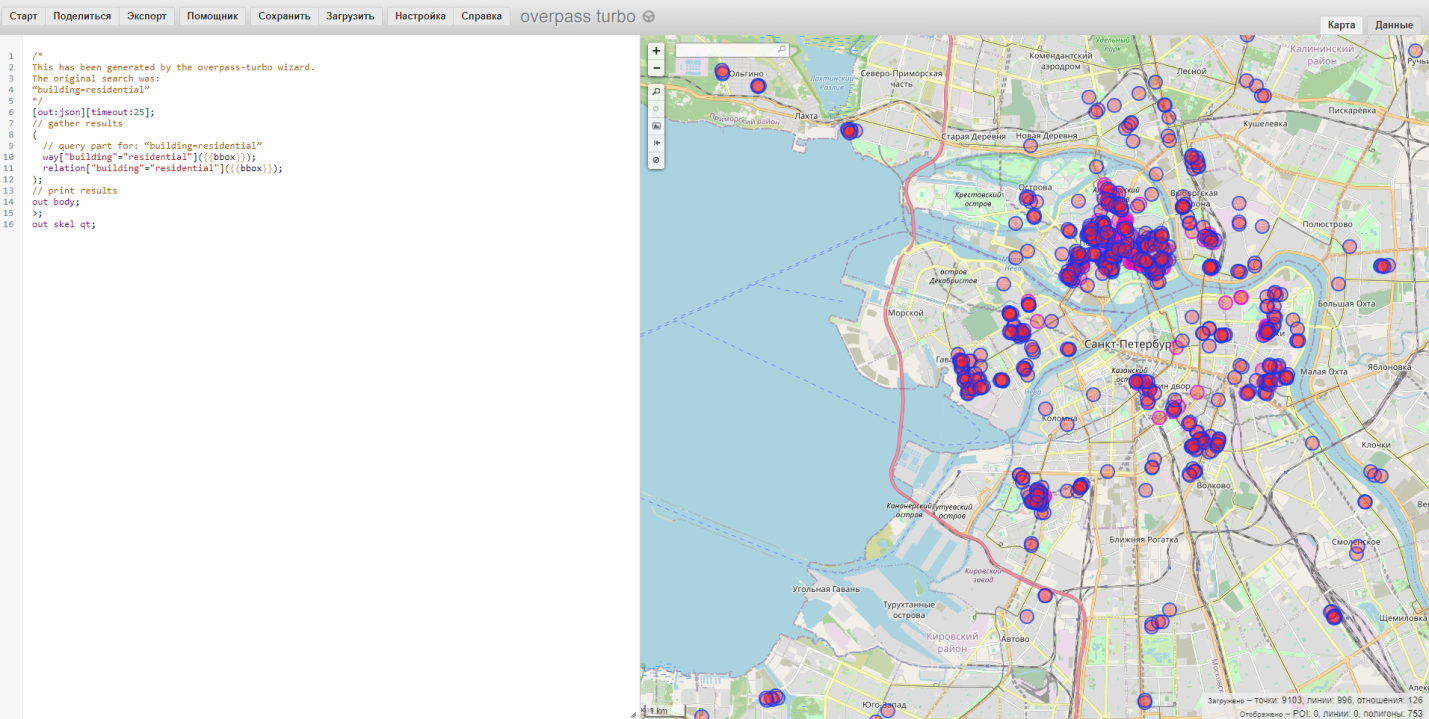
\includegraphics{figures/36.png}

Полученные объекты можно экспортировать в векторный формат данных geojson для дальнейшей работы в QGIS (кнопка Экспорт, загрузить как GeoJSON)

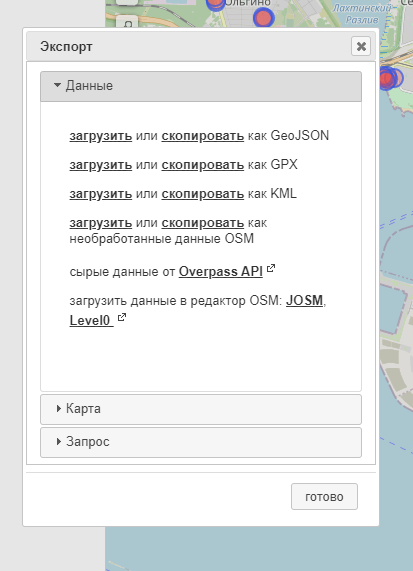
\includegraphics{figures/37.png}

Полученный файл можно открыть в QGIS~(в строке меню \emph{Слой -- Добавить слой -- Добавить векторный слой}).

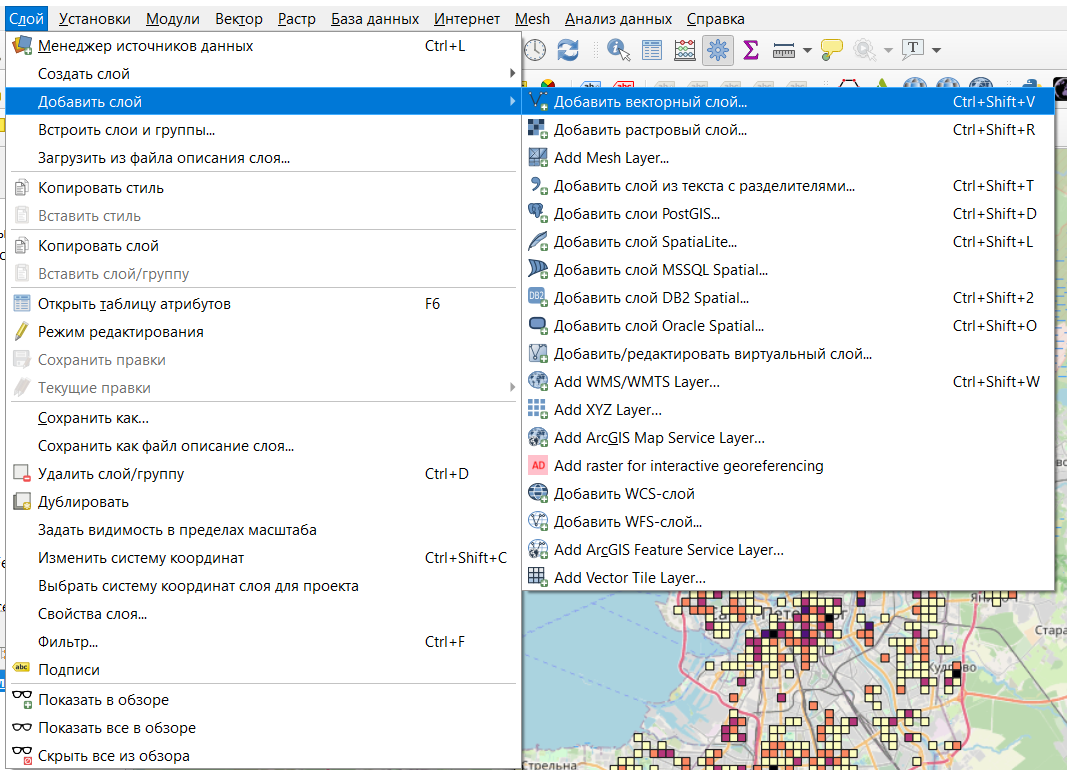
\includegraphics{figures/38.png}

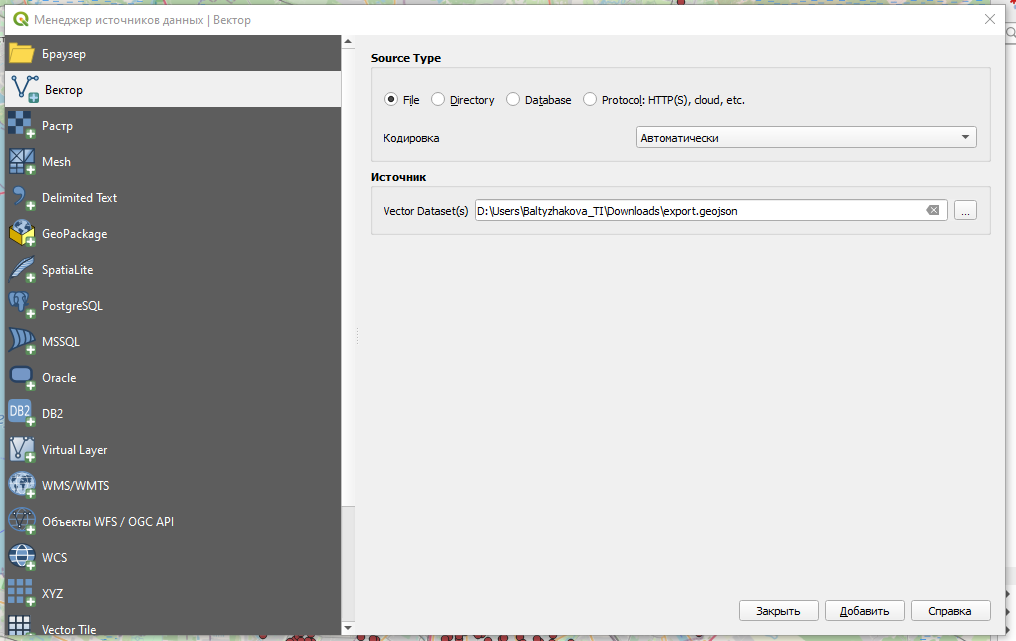
\includegraphics{figures/39.png}

В результате объекты должны появиться на вашей карте и в списке слоев.

\hypertarget{ux43eux43fux440ux435ux434ux435ux43bux435ux43dux438ux435-ux43fux43bux43eux449ux430ux434ux438-ux438-ux43fux435ux440ux438ux43cux435ux442ux440ux430-ux43eux431ux44aux435ux43aux442ux43eux432}{%
\chapter{Определение площади и периметра объектов}\label{ux43eux43fux440ux435ux434ux435ux43bux435ux43dux438ux435-ux43fux43bux43eux449ux430ux434ux438-ux438-ux43fux435ux440ux438ux43cux435ux442ux440ux430-ux43eux431ux44aux435ux43aux442ux43eux432}}

Определить площадь и периметр площадных объектов можно с помощью функции добавления геометрических параметров объектов к атрибутивной таблице или с помощью Калькулятора полей. Второй метод предпочтительнее, потому что меньше зависит от параметров системы координат.

Перед тем, как считать площадь нужно проверить единицы измерения, в которых будут проводиться расчеты. В строке меню нужно открыть настройки программы: Установки - Параметры. В открывшемся окне, нужно открыть Инструменты, где будут настройки инструментов измерения (Measure tools), в которых по умолчанию установлены единицы измерения расстояния - метры и единицы измерения - квадратные метры. При необходимости можно установить нужные единицы измерения.

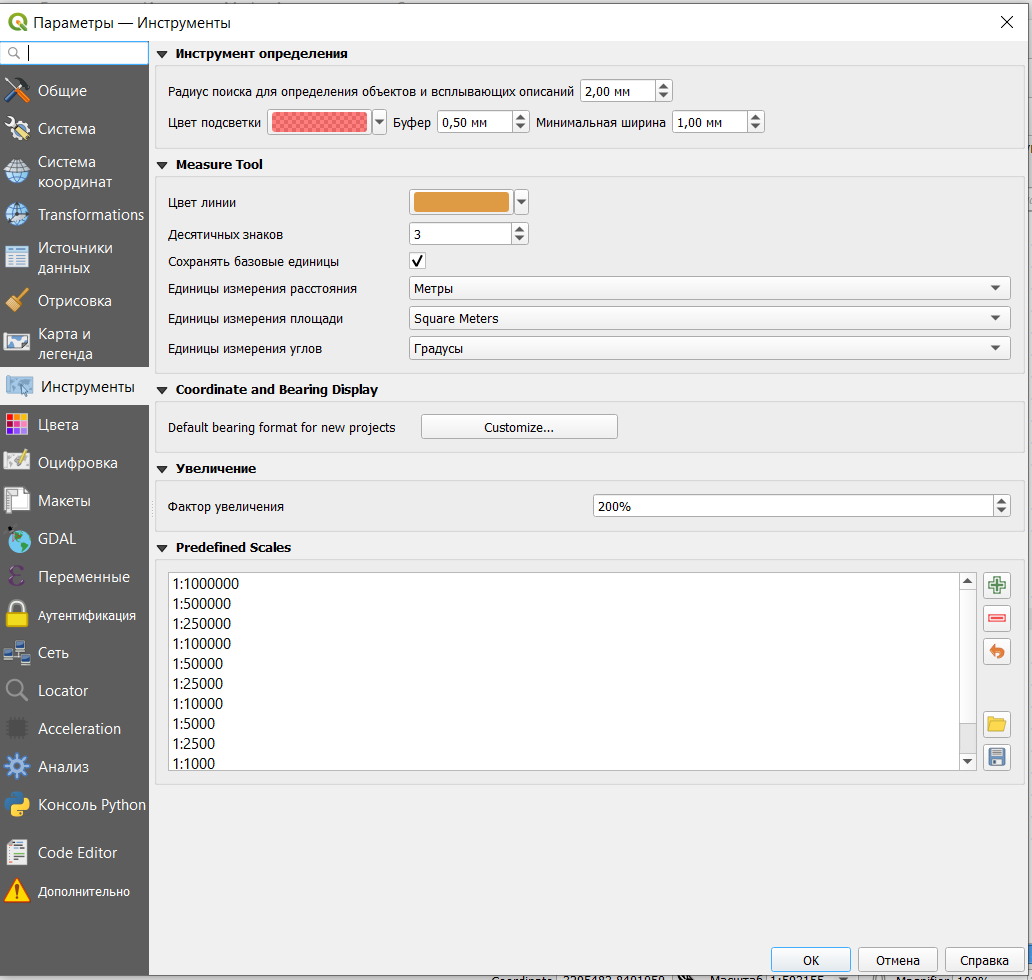
\includegraphics{figures/40.PNG}

Если~единицы измерения установлены правильные, то можно переходить к определению площади. Для этого нужно открыть таблицу атрибутов слоя.

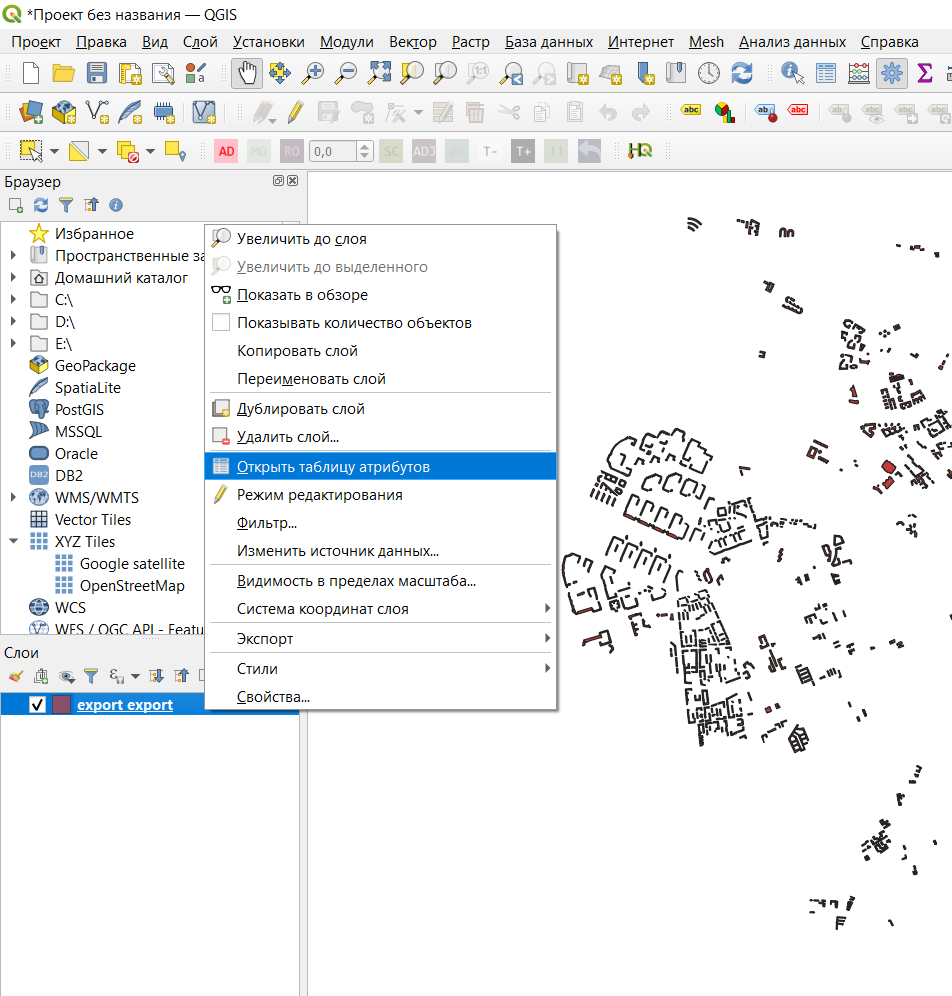
\includegraphics{figures/41.png}

В~таблице атрибутов нужно запустить Калькулятор полей (четвертый справа значок на панели инструментов).

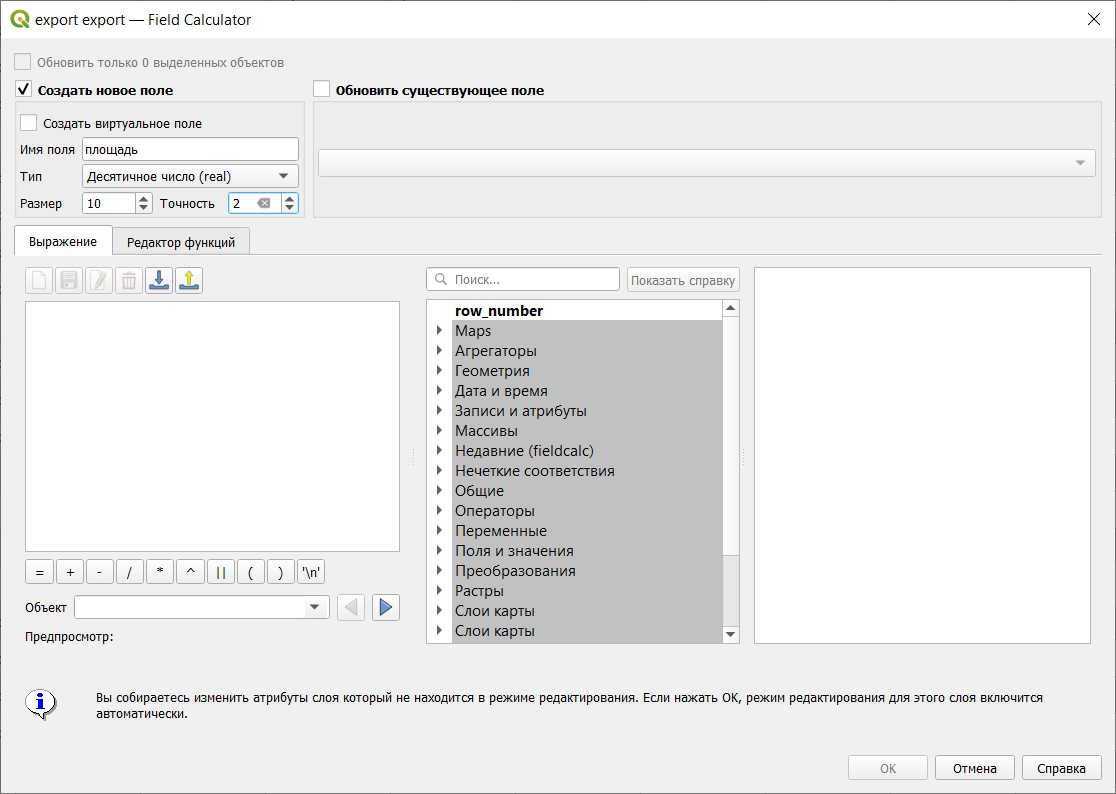
\includegraphics{figures/42.png}

Далее~нужно выбрать хотите ли вы записывать результат в новую колонку (поле) или внести в существующую. Мы запишем результаты в новое поле, для которого обязательно нужно указать имя и тип данных. Тип данных в данном случае нужен десятичное число с точностью (числом знаков после запятой) 2.

В нижней части калькулятора слева окно, в котором будет отображаться выражение, по которому осуществляются расчеты, посередине приведены все функции, которые можно использовать при расчетах, а справа - краткая справка по выбранной функции.

Для определения площади нужна функция \textbf{\$area}, входящая в группу Геометрия.

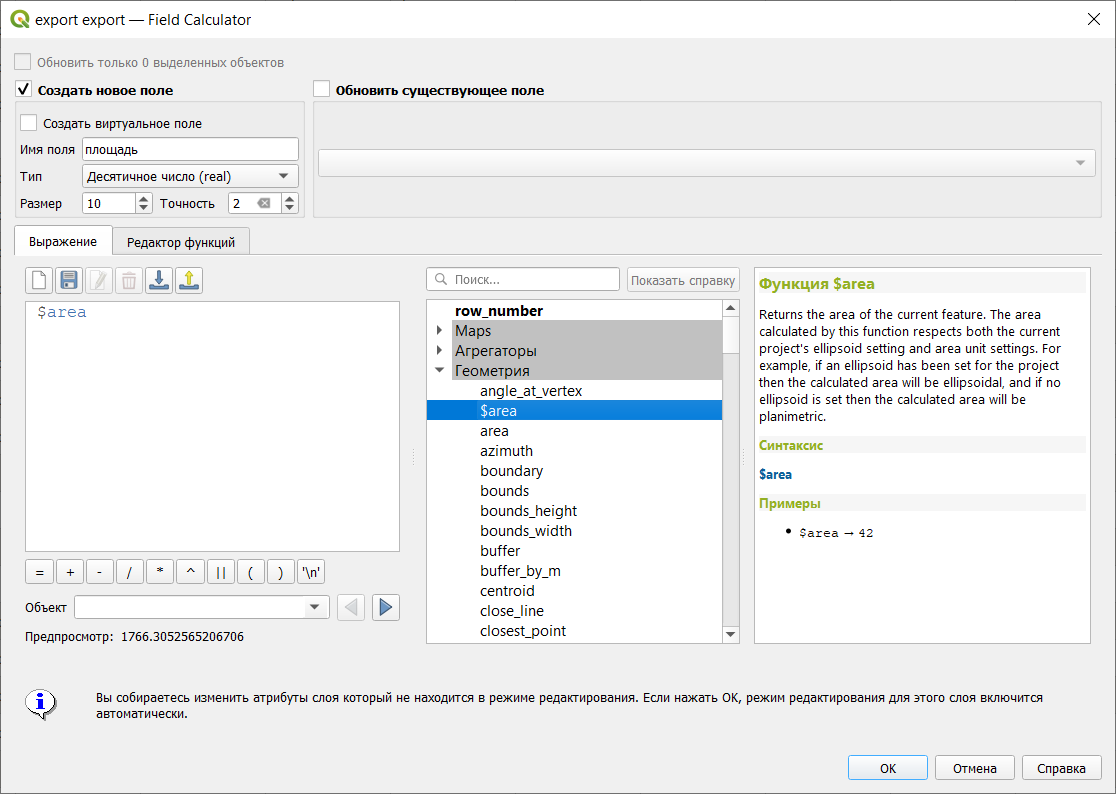
\includegraphics{figures/43.png}

После нажатия кнопки ОК, окно Калькулятора закроется, останется только окно таблицы атрибутов, в котором создана новая колонка с заданным именем и внесенными в нее значениями площади объектов.

Периметра рассчитывается аналогично, но с помощью функции \textbf{\$perimeter}.

Использования Калькулятора полей этим, конечно, не ограничивается: с его помощью можно осуществлять различные вычисления между атрибутами ваших объектов.

\hypertarget{ux43fux43eux441ux442ux440ux43eux435ux43dux438ux435-ux431ux443ux444ux435ux440ux43dux44bux445-ux437ux43eux43d-ux438-ux43eux432ux435ux440ux43bux435ux439ux43dux44bux435-ux43eux43fux435ux440ux430ux446ux438ux438}{%
\chapter{Построение буферных зон и оверлейные операции}\label{ux43fux43eux441ux442ux440ux43eux435ux43dux438ux435-ux431ux443ux444ux435ux440ux43dux44bux445-ux437ux43eux43d-ux438-ux43eux432ux435ux440ux43bux435ux439ux43dux44bux435-ux43eux43fux435ux440ux430ux446ux438ux438}}

\hypertarget{ux431ux443ux444ux435ux440ux43dux44bux435-ux437ux43eux43dux44b}{%
\section{Буферные зоны}\label{ux431ux443ux444ux435ux440ux43dux44bux435-ux437ux43eux43dux44b}}

Буферизация~обычно создает две области: одна~в пределах~ указанного расстояния от выбранного объекта реального мира, другая - вне. Область, которая находится в пределах указанного расстояния называется~буферная зона.

С помощью буферных зон может осуществляться построение радиусов обслуживания определенных объектов, радиусов распространения отдельных явлений, границ зон с особыми условиями использования территорий.

Для создания буферной зоны необходимо убедиться, что проекция слоя позволяет измерение длин в метрической системе измерений, то есть в метрах. При необходимости слой нужно либо перепроецировать одноименным инструментом из панели инструментов анализа, либо просто пересохранить из контекстного меню слоя в нужной проекции командой \emph{Сохранить как}.

Предположим, что нам нужно определить, какие дома обслуживаются магазинами, а какие нет. Установим радиус обслуживания магазинов 150 метров.

В нашем случае мы строим буферы вокруг магазинов, для которых система координат подразумевает измерения ~в градусах, поэтому размер буфера мы сможем задать только в градусах.

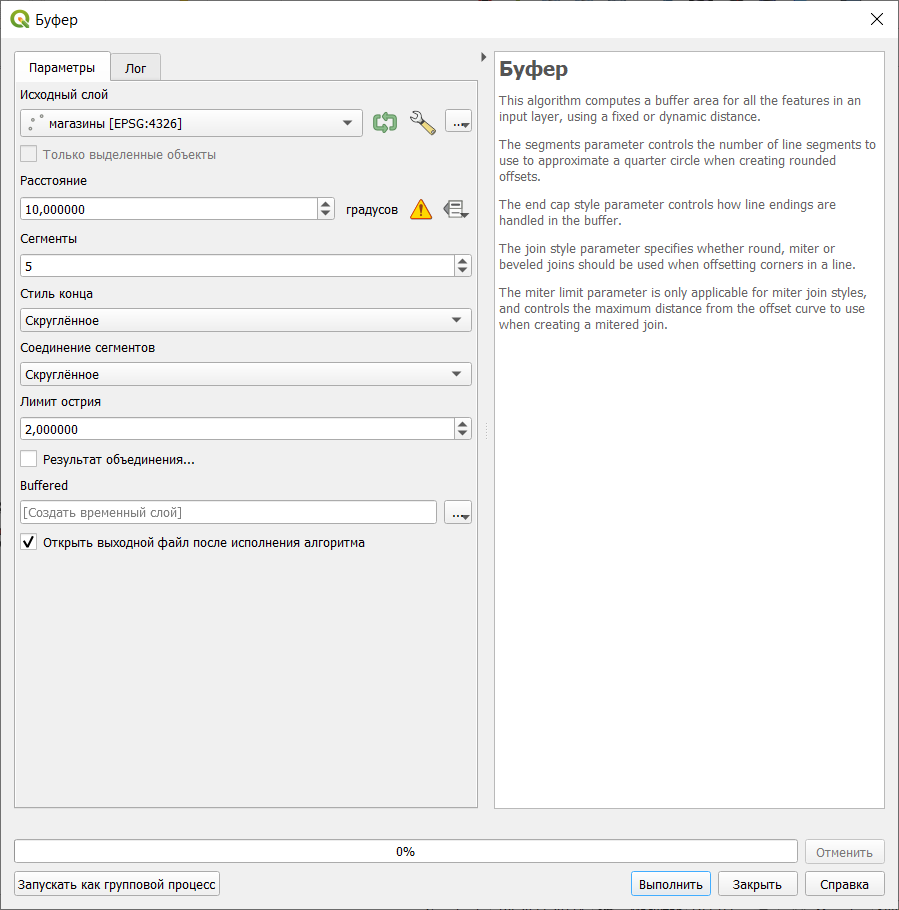
\includegraphics{figures/44.png}

Чтобы задавать размер буфера в метрах, нам нужно сначала перепроецировать исходный слой с помощью инструмента \emph{Перепроецировать слой}. В качестве целевой системы координат можно выбрать системы \texttt{EPSG:3857}, результаты лучше сохранить в файл.

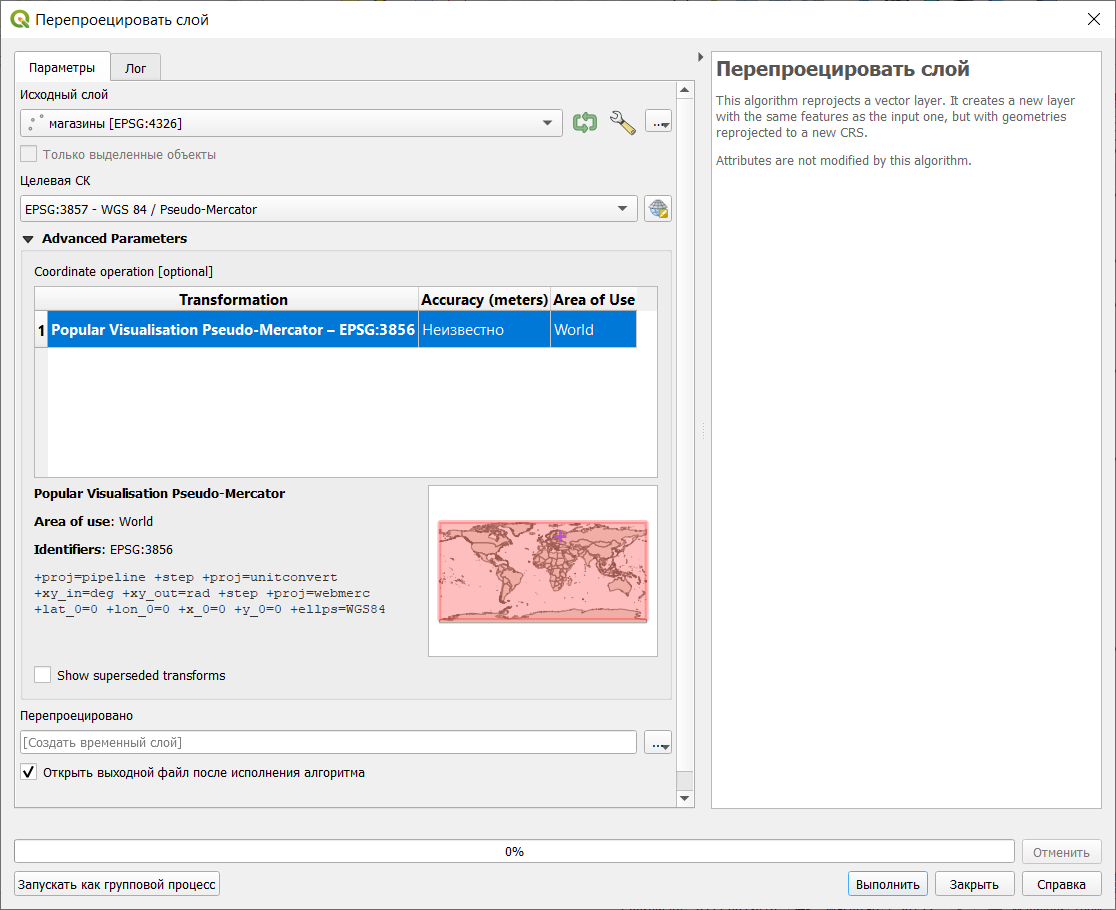
\includegraphics{figures/45.png}

Новый перепроецированный слой будет отличаться от исходного только системой координат.

Далее мы можем создать буферы размером 150 метров для магазинов на основе перепроецированного слоя (результаты лучше тоже сохранить в файл).

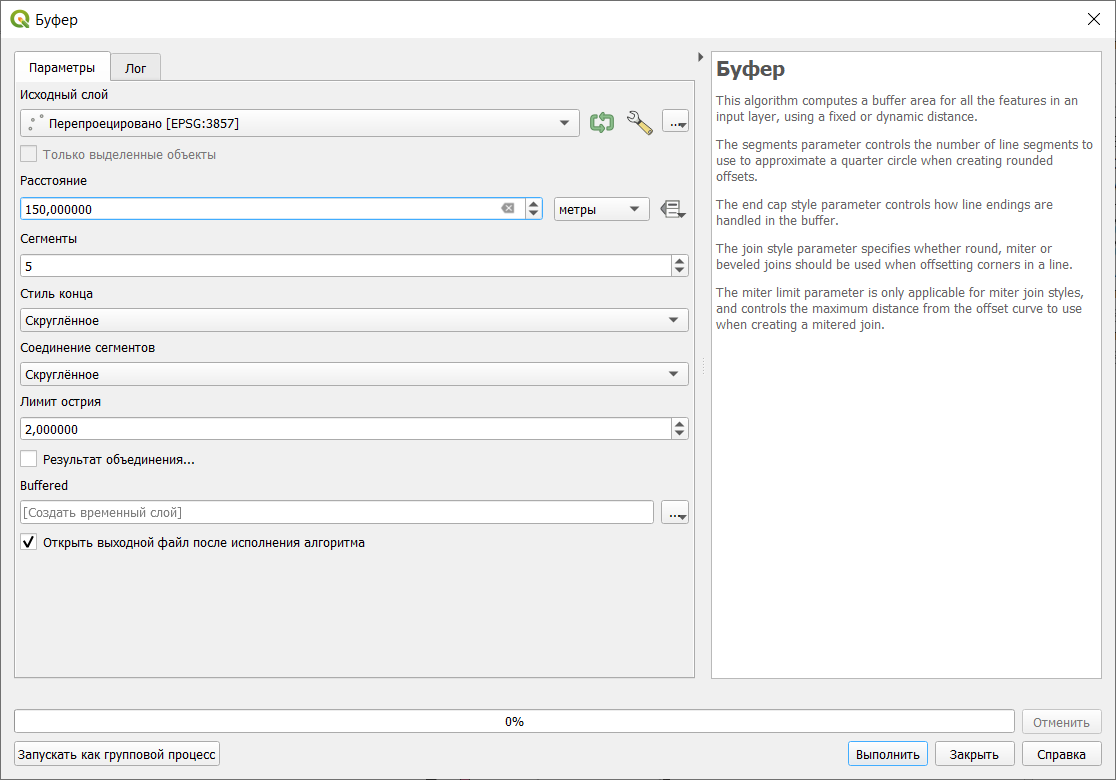
\includegraphics{figures/46.png}

В результате должны получиться круги заданного радиуса вокруг магазинов.

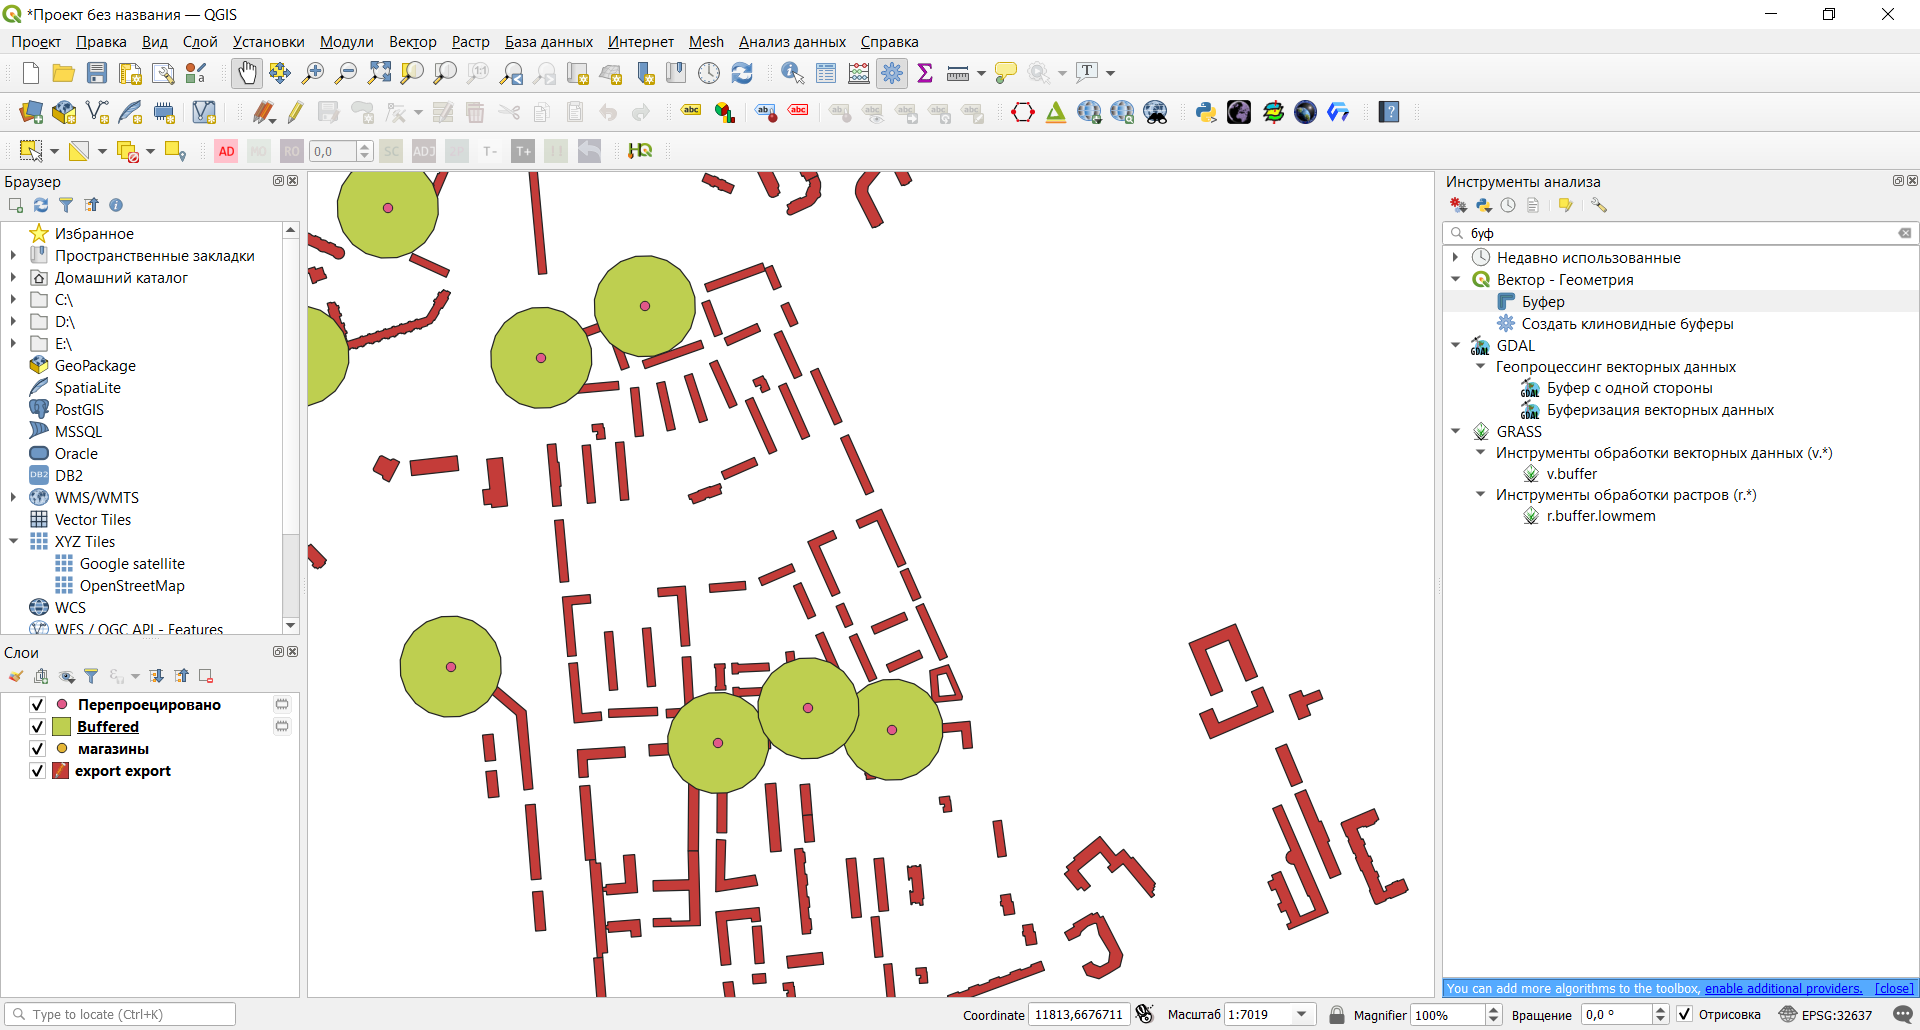
\includegraphics{figures/47.png}

\hypertarget{ux43fux43eux438ux441ux43a-ux43eux431ux44aux435ux43aux442ux43eux432-ux43fux43eux43fux430ux434ux430ux44eux449ux438ux445-ux432-ux440ux430ux434ux438ux443ux441-ux43eux431ux441ux43bux443ux436ux438ux432ux430ux43dux438ux44f}{%
\section{Поиск объектов, попадающих в радиус обслуживания}\label{ux43fux43eux438ux441ux43a-ux43eux431ux44aux435ux43aux442ux43eux432-ux43fux43eux43fux430ux434ux430ux44eux449ux438ux445-ux432-ux440ux430ux434ux438ux443ux441-ux43eux431ux441ux43bux443ux436ux438ux432ux430ux43dux438ux44f}}

Далее мы можем осуществить поиск домов, которые попадают в заданные области обслуживания.

Для поиска объектов есть группа инструментов \emph{Вектор-Выбор}.

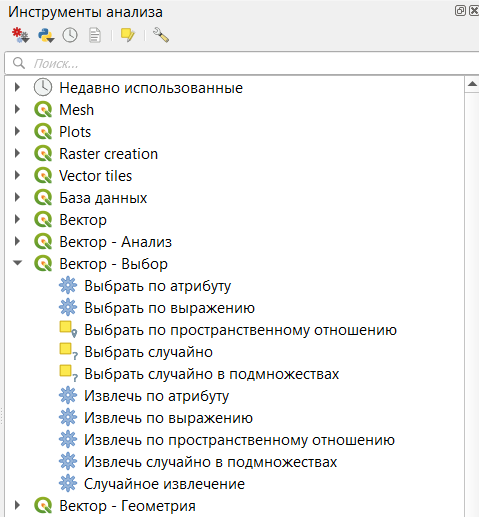
\includegraphics{figures/48.png}

Часть инструментов в ней начинается со слова Выбрать, а часть - Извлечь. Разница между ними в том, что в первом случае объекты просто выделяются в исходном слое, а во втором - объекты, соответствующие заданным условия, извлекаются в новый слой.

Краткое описания инструментов:

\begin{itemize}
\item
  выбрать\textbackslash извлечь по атрибуту - поиск объектов по значению одного из атрибутов;
\item
  выбрать\textbackslash извлечь по выражению - поиск объектов по значениям нескольких атрибутов одновременно;
\item
  выбрать\textbackslash извлечь по пространственному отношению - поиск объектов по их расположению относительно объектов другого слоя;
\item
  выбрать\textbackslash извлечь случайно - случайная выборка объектов из слоя (заданного числа объектов или заданного процента объектов);
\item
  выбрать\textbackslash извлечь случайно в подмножествах - сначала слой разбивается по категориям по одному из атрибутов, потом из каждой категории извлекается заданное число или заданный процент объектов.
\end{itemize}

Нам ~нужно определить, какие здания попадаются в буферные зоны, поэтому нужно воспользоваться выбрать\textbackslash извлечь по пространственному отношению.

Для выбора объектов нужно сначала указать в каком слое осуществляется поиск (слой со зданиями), геометрический оператор (как объекты расположены относительно объектов другого слоя) и слой для сравнения (буферные зоны). Геометрические операторы в данном случае лучше выбирать \emph{Пересекает} и \emph{В пределах}.

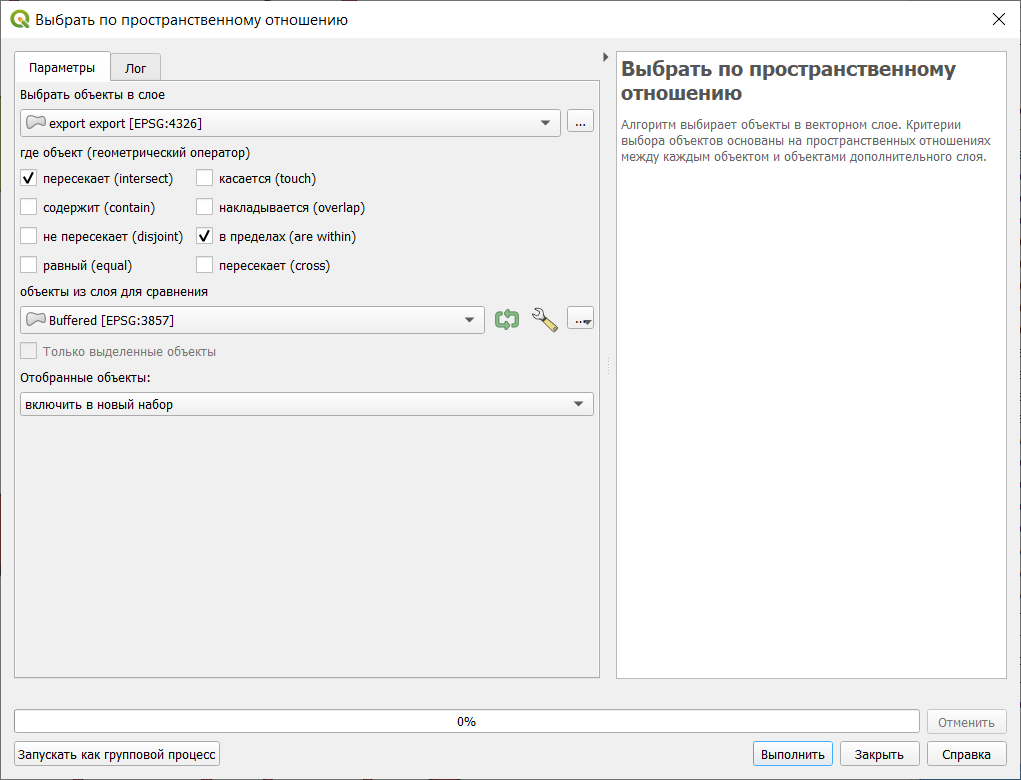
\includegraphics{figures/49.png}

В результате выбранные объекты будут выделены желтым цветом на карте.

\includegraphics{figures/50.png}

Функция Извлечь по пространственному отношению работает аналогично с почти теми же характеристиками, кроме того, что вы можете выбрать сохранить результаты во временный слой или в файл.

\includegraphics{figures/51.png}

В результате вы получите новый слой, в котором будут содержаться только те объекты, которые соответствуют заданному условию.

\includegraphics{figures/52.png}

\hypertarget{ux43eux432ux435ux440ux43bux435ux439ux43dux44bux435-ux43eux43fux435ux440ux430ux446ux438ux438}{%
\section{Оверлейные операции}\label{ux43eux432ux435ux440ux43bux435ux439ux43dux44bux435-ux43eux43fux435ux440ux430ux446ux438ux438}}

Оверлейные операции являются одним из основных способов пространственного анализа. Название этих операций произошло от слова overlay - наложение. Суть оверлейных операций состоит в том, что два слоя накладываются друг на друга, после чего осуществляется какая-то операция (разность, обрезка и т.п.) в результате чего создается результирующий новый слой.

В QGIS можно выполнить следующие оверлейные операции:~\emph{Обрезать, Пересечение,~Объединение,~Симметричная разность,~Разность}.

Проиллюстрирую работу различных операций на основе буферных зон вокруг магазинов (500 м) и квадратов сетки.

Исходные слои

\includegraphics{figures/53.PNG}

При выполнении команды \emph{Пересечение} в выходном слое содержатся только участки, в которых оба слоя пересекаются.

\includegraphics{figures/54.PNG}

Команда~\emph{Объединение}~совмещает слои таким образом, что в выходном слое содержатся как участки пересечения, так и участки, принадлежащие только одному из слоев.

\includegraphics{figures/55.PNG}

Команда~\emph{Симметричная~разность} оставляет в выходном слое только те участки, в которых исходные слои не пересекаются.

\includegraphics{figures/56.PNG}

Команда~\emph{Обрезать}~совмещает слои таким образом, что в выходном слое содержатся только те участки, которые пересекаются со слоем отсечения. Принципиальное отличие этой команды от пересечения в том, что сохраняется исходная геометрия объектов, тогда как при пересечении исходные объекты дополнительно рассекаются объектами накладывающегося слоя.

\includegraphics{figures/57.PNG}

Команда~\emph{Разность}~совмещает слои таким образом, что в выходном слое содержатся только те участки, которые не пересекаются со слоем отсечения.

\includegraphics{figures/58.PNG}

\begin{quote}
Важно помнить, что результат оверлейных операций зависит от того, какой слой будет указан первым (будет исходным), а какой вторым (будет накладываться). В приведенных примерах везде слой буферных зон был исходным, а накладывался слой с сеткой.
\end{quote}

Все оверлейные операции находятся с панели инструментов в группе Вектор-Оверлей. Подробнее~с примерами можно прочесть \href{https://docs.qgis.org/3.10/ru/docs/user_manual/processing_algs/qgis/vectoroverlay.html}{\underline{https://docs.qgis.org/3.10/ru/docs/user\_manual/processing\_algs/qgis/vectoroverlay.html}}

\hypertarget{ux440ux430ux431ux43eux442ux430-ux441ux43e-ux441ux43bux43eux44fux43cux438-ux432-ux43aux43eux442ux43eux440ux44bux445-ux435ux441ux442ux44c-ux432ux440ux435ux43cux435ux43dux43dux430ux44f-ux441ux43eux441ux442ux430ux432ux43bux44fux44eux449ux430ux44f}{%
\chapter{Работа со слоями, в которых есть временная составляющая}\label{ux440ux430ux431ux43eux442ux430-ux441ux43e-ux441ux43bux43eux44fux43cux438-ux432-ux43aux43eux442ux43eux440ux44bux445-ux435ux441ux442ux44c-ux432ux440ux435ux43cux435ux43dux43dux430ux44f-ux441ux43eux441ux442ux430ux432ux43bux44fux44eux449ux430ux44f}}

Кроме обычных пространственных данных QGIS~позволяет работать с данными, в которых есть сведения о дате и времени.

Это задание лучше сделать в отдельном пустом проекте. Исходные данные нужно скачать с сайта \href{https://how-old-is-this.house/}{\underline{https://how-old-is-this.house/}}~в разделе Данные~(для любого из городов). Скачанные данные нужно обязательно распаковать, а потом открыть файл (в строке меню \emph{Слой -- Добавить слой -- Добавить векторный слой}).

В~этом слое есть два поля с данными о годе постройки: r\_year\_string (текстовое поле), r\_year\_int~(целое число). Но для нас обязательно нужно поле с типом данных Дата. Для этого сделаем новую колонку из имеющихся с помощью калькулятора полей.

Для этого воспользуемся функцией ~to\_date, которая преобразует данные в формат даты. В качестве параметров здесь обязательно нужно указать, какое поле преобразуется и в какой формат даты. В нашем случае выражение будет выглядеть так: ~\textbf{to\_date( r\_year\_int,`yyyy')}

\includegraphics{figures/59.png}

В результате в таблице атрибутов будет добавлено поле, в котором даты будут приведены примерно так: 1991-01-01 (первое января в нашем случае, потому что день и месяц неизвестны).

Но не для всех домов у нас есть год постройки, поэтому отфильтруем только те дома, для которых год известен.

Фильтр для слоя открывается из контекстного меню, которое вызывается нажатием правой кнопки мыши на название слоя. Так как слой находится в режиме редактирования, фильтр неактивен, поэтому сначала в контекстном меню нужно сначала нажать Режим редактирования, чтобы его отключить (изменения нужно сохранить).

\includegraphics{figures/60.png}

Далее нужно поменять настройки слоя, чтобы он распознавался как слой, содержащий характеристики времени. Для этого нужно открыть Свойства слоя, параметр Временные данные.

\includegraphics{figures/61.png}

Для начала нужно поставить галочку напротив слов Временные данные, потом выбрать тип данных (configuration), в нашем случае - это поле с датой\textbackslash временем (single field with date\textbackslash time), после этого нужно выбрать поле, содержащее дату, задать продолжительность событий (event duration) в 1 год и указать, что объекты со временем накапливаются в слое (accumulate features over time).

После применения свойств напротив названия слоя должны быть два значка: воронка (фильтр) и циферблат (временные данные). Далее нужно запустить Temporal controller - панель для работы с временными данными. Открыть панель можно через строку меню: \emph{Вид - Панели - Temporal controller}.

После этого появится серая горизонтальная панель, в которой можно настроить анимированное отображение данных по времени.

\includegraphics{figures/62.png}

\hypertarget{ux438ux43dux442ux435ux440ux43fux43eux43bux44fux446ux438ux44f}{%
\chapter{Интерполяция}\label{ux438ux43dux442ux435ux440ux43fux43eux43bux44fux446ux438ux44f}}

Интерполяция - это восстановление значений непрерывной величины по имеющимся дискретным значениям. Например, определены высоты в определенных точках, по которым осуществляется интерполяция, для того, чтобы получить значения высот на всех рассматриваемой местности.

Наиболее распространенными и широко применяемыми являются два метода интерполяции: \emph{TIN-интерполяция (Triangulated Irregular Network) и метод обратно взвешенных расстояний}.

В первом методе на основе исходных точек сначала строится сеть треугольников - триангуляция Делоне, в которой соединяются между собой соседние точки. Далее по полученным треугольникам осуществляется интерполяция.

Главным недостатком этого метода является то, что в результате получается негладкая поверхность. Однако именно этот метод, как правило, рекомендуют применять для рельефа и высот, так как в этом случае исходны точки играют роль характерных точек рельефа.

В методе обратно взвешенных расстояний всем точкам присваиваются веса в зависимости от того, как далеко они расположены от той точки, для которой выполняется интерполяция. Принимается, что далеко расположенные точки мало влияют друг на лруга и на значения в искомой точке, а близко расположенные - оказывают сильное влияние. Этот метод позволяет получить довольно гладкую результирующую поверхность и его рекомендуют применять для всех характеристик кроме рельефа.

В результате интерполяции получается растровое изображение, в каждой ячейке которого содержится значения интерполируемой величины.

Основными параметрами при TIN-интерполяции являются исходный слой, параметр интерполяции, охват слоя и параметры выходного растра.

\includegraphics{figures/63.png}

Основными параметрами при интерполяции методов обратно взвешенных расстояний являются исходный слой, параметр интерполяции, охват слоя и параметры выходного растра, а также коэффициент расстояния, который влияет на присваиваемые веса точек. Чем больше величина коэффициента расстояния, тем более дискретные значения будут получены.

\includegraphics{figures/64.png}

Полученный растр можно использовать для построения трехмерной поверхности.

\hypertarget{ux446ux438ux444ux440ux43eux432ux44bux435-ux43cux43eux434ux435ux43bux438-ux440ux435ux43bux44cux435ux444ux430}{%
\chapter{Цифровые модели рельефа}\label{ux446ux438ux444ux440ux43eux432ux44bux435-ux43cux43eux434ux435ux43bux438-ux440ux435ux43bux44cux435ux444ux430}}

\hypertarget{ux43cux43eux440ux444ux43eux43cux435ux442ux440ux438ux447ux435ux441ux43aux438ux439-ux430ux43dux430ux43bux438ux437-ux440ux435ux43bux44cux435ux444ux430}{%
\section{Морфометрический анализ рельефа}\label{ux43cux43eux440ux444ux43eux43cux435ux442ux440ux438ux447ux435ux441ux43aux438ux439-ux430ux43dux430ux43bux438ux437-ux440ux435ux43bux44cux435ux444ux430}}

Цифровые модели рельефа, как правило, строят либо по результатам интерполяции, либо на основе открытых данных.

Самым распространенным источником данных о рельефе является цифровая модель рельефа SRTM (shuttle radar topographic mission). Эта цифровая модель была получена в 2000 году на основе спутниковой радарной съемки. Она охватывает планету между 54 градусами южной широты и 60 градусами северной широты. Подробнее на русском можно почитать про нее \href{https://gis-lab.info/qa/srtm.html}{здесь}

Скачать данные SRTM можно на сайте Геологической службы США (\url{https://earthexplorer.usgs.gov/}) или с помощью плагина SRTM downloader.

Для примера и выполнения работы были скачаны данные для окрестностей Эльбруса. Они находятся \href{https://drive.google.com/file/d/1s57yc3rKQbZfFcM8TeWsI6t6HCc7412w/view?usp=sharing}{здесь}.

В каждой ячейке исходного растрового изображения содержится значение высоты.

Добавление растрового слоя осуществляется через строку меню \textbf{Слой - Добавить слой - Добавить растровый слой}.

\includegraphics{figures/65.png}

В результате должно появиться изображение рельефа в оттенках серого цвета.

\includegraphics{figures/66.PNG}

Это изображение можно сделать цветным, для этого нужно открыть свойства слоя. В настройках стиля нужно выбрать тип изображения \emph{Одноканальное псевдоцветно}е.

\includegraphics{figures/67.PNG}

Градиент можно создать самостоятельно с помощью редактора.

В результате будет получено изображение растра в цветах выбранного градиента.

\includegraphics{figures/68.PNG}

С использованием такого растра может быть построена трехмерная поверхность, отображающая рельеф местности, а также выполнен ряд вычислений для морфометрического анализа рельефа. Для более наглядного отображения рельефа на карте рассчитывается теневой рельеф, который строится с использованием позиции источника направленного света.

\includegraphics{figures/69.png}

В результате должно получиться что-то подобное.

\includegraphics{figures/70.PNG}

Этот теневой рельеф можно использовать, чтобы добавить дополнительный объем подложке или исходному рельефу растра. Для этого нужно открыть свойства слоя с теневым рельефом и изменить режим смешивания на Добавление или Осветление (также можно поэкспериментировать с настройками яркости и контрастности).

\includegraphics{figures/71.PNG}

Поверх исходного растра с рельефом получается подобный результат.

\includegraphics{figures/72.PNG}

Рассчитаем крутизну склонов.

\includegraphics{figures/73.png}

Так как на рассматриваемой местности довольно крутые склоны, лучше их считать в процентах, а не в градусах (Slope expressed as percent instead of degrees).

\includegraphics{figures/74.PNG}

Результат определения крутизны склонов.

\includegraphics{figures/75.PNG}

Это изображение мы также можем сделать цветным и наложить на него теневой рельеф для большего объема.

Определим экспозицию склонов - ориентацию по сторонам света.

\includegraphics{figures/76.png}

\includegraphics{figures/77.PNG}

Результат в цветном виде с наложенным поверх теневым рельефом.

\includegraphics{figures/78.PNG}

Рассмотрим рельеф как трехмерную поверхность. Чтобы открыть трехмерный вид карты, нужно в строке меню выбрать \textbf{Вид- Новая 3D карта}. В данном случае была добалвена подложка со спутниковым изображением с теневым рельефом поверх.

\includegraphics{figures/79.PNG}

Трехмерный вид открывается в отдельном окне программы, но если его повращать, то станет заметно, что карта все еще плоская. Чтобы поверхность стала трехмерной нужно нажать кнопку Configure\ldots{} и выбрать тип DEM (raster layer), высота должна браться из исходного растра.

\includegraphics{figures/80.PNG}

Полученная поверхность

\includegraphics{figures/81.PNG}

\hypertarget{ux441ux43eux437ux434ux430ux43dux438ux435-ux433ux43eux440ux438ux437ux43eux43dux442ux430ux43bux435ux439}{%
\section{Создание горизонталей}\label{ux441ux43eux437ux434ux430ux43dux438ux435-ux433ux43eux440ux438ux437ux43eux43dux442ux430ux43bux435ux439}}

Из растра со значениями высот могут быть извлечены горизонтали

\includegraphics{figures/82.png}

Расстояние между изолиниями - это фактически высота сечения рельефа, то есть через сколько мы будем проводить горизонтали.

\includegraphics{figures/83.PNG}

Полученные изолинии

\includegraphics{figures/84.PNG}

Настроим горизонтали таким образом, чтобы каждая пятая была утолщенной, добавим подписи и настроим их так, чтобы они были ``головой вверх''.

Начнем с настройки толщины линий. Для этого в свойствах слоя выберем настройку толщины в зависимости от выражения.

\includegraphics{figures/85.png}

Далее пропишем логическое выражение: \textbf{if(``ELEV''\%500=0,0.7,0.3)}. В этом выражении перед запятой прописано условие - высота горизонтали делится на 500 без остатка, потом толщина линии, если условие выполняется, и толщина, если условие не выполняется.

\includegraphics{figures/86.PNG}

Результат

\includegraphics{figures/87.PNG}

Добавим подписи.

\includegraphics{figures/88.PNG}

Но при таком добавлении подписей, будут подписаны все горизонтали, а мы хотим подписать только утолщенные. Для этого нужно прописать выражение, подобное тому, что мы писали выше: \textbf{if(``ELEV''\%500=0,``ELEV'',"").}

\includegraphics{figures/89.PNG}

Добавим белую обводку подписям, чтобы они не сливались с горизонталями

\includegraphics{figures/90.PNG}

Сделаем так, чтобы они размещались на линии и изгибались в соответствии с ней.

\includegraphics{figures/91.PNG}

И настроим подписи так, чтобы все они смотрели головой в сторону увеличения высоты.

\includegraphics{figures/92.PNG}

\includegraphics{figures/93.PNG}

В результате получим горизонтали, где каждая пятая будет утолщена и подписана головой в сторону увеличения.

\includegraphics{figures/94.PNG}

\end{document}
